\documentclass[iop]{emulateapj-rtx4}


%\documentclass[12pt]{article}
%\pdfpagewidth 8.5in
%\pdfpageheight 11in 
%\setlength\topmargin{0in}
%\setlength\headheight{0in}
%\setlength\headsep{0in}
%\setlength\textheight{9in}
%\setlength\textwidth{6.5in}
%\setlength\oddsidemargin{0in}
%\setlength\evensidemargin{0in}

\usepackage{graphicx}
\usepackage{amssymb}

%\usepackage{multicol}
%\usepackage{sidecap}
%\usepackage{ragged2e}

%\usepackage{caption}
%\usepackage{subcaption}

%\usepackage{subfig}
\usepackage{wrapfig}
\usepackage{setspace}
\usepackage{subfigure}
\usepackage{mathtools}


%\newcommand{\rms}[1]{\langle #1 \rangle}
%\renewcommand{\baselinestretch}{1.5}
%\renewcommand{\thefootnote}{\roman{footnote}}

\graphicspath{{paper_figures4//}}


\frenchspacing

\begin{document}

%\onehalfspacing

%\title{A Dichotomy in the Relative Velocity of Ly$\alpha$ Absorption in Nearby Galaxy Halos}
\title{Matching Ly$\alpha$ Absorption to Nearby Galaxy Halos with a Likelihood-based Method\textsuperscript{*}}

%\footnote{\rm{This research has made use of the NASA/IPAC Extragalactic Database (NED) which is operated by the Jet Propulsion Laboratory, California Institute of Technology, under contract with the National Aeronautics and Space Administration.}}

\author{David M. French, Bart P. Wakker}
\affil{Department of Astronomy, University of Wisconsin - Madison}

%\affil{Department of Astronomy, University of Wisconsin - Madison; frenchd@astro.wisc.edu}


\begin{abstract}

We present initial results from an ongoing large-scale study of the circumgalactic medium in the nearby Universe ($cz \leq 10,000$ km/s), using archival Cosmic Origins Spectrograph (COS) spectra of background QSOs. This initial sample contains 35 sight lines chosen for their proximity to large galaxies ($D\geq25$ kpc) and high signal-to-noise ratio (S/N $\geq$ 11), yielding 51 Ly$\alpha$ systems which we have paired with individual galaxies. We introduce a likelihood parameter to facilitate the matching of galaxies to absorption lines in a reproducible manner. We find the usual anti-correlation between Ly$\alpha$ equivalent width ($EW$) and impact parameter ($\rho$) when we normalize by galaxy virial radius ($R_{vir}$). Galaxies associated with a Ly$\alpha$ absorber are found to be more highly-inclined than the average distribution of galaxies in the survey volume at a $>99\%$ confidence limit. Contrary to suggestions in other recent papers, we do not see obvious correlations with azimuth angle. 

%We also detect a slight dichotomy in the equivalent widths of absorption systems around $\Delta v = v_{galaxy} - v_{gas}$, with positive $\Delta v$ absorption median $EW$ = $288 \pm 15$ m\AA, and negative $\Delta v$  absorption median $EW$ = $177 \pm 10$ m\AA, but have not yet been able to explain this finding. 

%This $W$ difference is significant at a greater than $99\%$ confidence limit. We also find a positive correlation between absorber-galaxy impact parameter and galaxy $R_{vir}$, a preference for absorption around highly inclined galaxies, but little evidence of azimuthal dependence.


%Galaxies must accrete gas from the intergalactic medium (IGM) in order to sustain star formation at observed levels. In order to understand this complex process, and how it influences galaxy evolution, it is necessary to understand the physical conditions and distribution of the gas around galaxies, known as the circumgalactic medium (CGM). For my thesis, I propose to use archival spectra of bright background QSOs taken by the Cosmic Origins Spectrograph (COS) on the Hubble Space Telescope (HST) to directly probe the CGM of galaxies in the nearby Universe. I will supplement this spectral data with observations of these galaxies taken by the WIYN and SALT telescopes. This proposed program will be the largest and most statistically significant survey of the local CGM to date.

\end{abstract}
\keywords{IGM, CGM, galaxies}


\footnotetext[*]{This research has made use of the NASA/IPAC Extragalactic Database (NED) which is operated by the Jet Propulsion Laboratory, California Institute of Technology, under contract with the National Aeronautics and Space Administration. 
Based on observations with the NASA/ESA \textit{Hubble Space Telescope}, obtained at the Space Telescope Institute, which is operated by AURA, Inc., under NASA contract NAS 5-26555.}


%\section{THINGS I STILL NEED}
%
%- galaxy table completeness plot
%- breakdown of systems into single galaxy (certain), multiple galaxies (probable), multiple galaxies (ambiguous)
%- mean Lstar for associated galaxies of each type


\section{Introduction}

It is well known that galaxies must continue to accrete gas throughout their lifetimes in order to sustain their observed levels of star formation (e.g. Erb 2008, Putman et al. 2009b). This additional gas must come from the diffuse intergalactic medium (IGM), where the majority of the baryons in the universe reside (Penton et al. 2002, 2004; Lehner et al. 2007; Danforth $\&$ Shull 2008; Shull et al. 2012). How exactly this IGM gas eventually falls into the halos and disks of galaxies is still highly uncertain, as observational constraints are hard to come by. Because of the diffuse nature of IGM gas it is most readily and sensitively detected as absorption in the spectra of background active galactic nuclei (AGN). The advent of the sensitive UV spectrographs STIS and COS on the Hubble Space Telescope (HST) has provided a wealth of information on the properties and distribution of both the ions of heavy elements as well as the Lyman series of neutral H\,{\sc i} gas around galaxies. 

Individual concentrations of gas along a given sightline imprint absorption lines on the spectrum in the direction of the QSO. The metal lines trace the star formation history within the intervening gas, and neutral hydrogen lines (Ly$\alpha$) indicate both the location and velocities of outflowing gas, as well as the presence of fuel for future star formation. Numerous studies using these observations have shown that many Ly$\alpha$ absorbers trace individual galaxy halos (e.g. Lanzetta et al 1995, Tripp et al. 1998, Chen et al. 1998, 2001a, Wakker $\&$ Savage 2009, Steidel et al. 2010, Prochaska et al. 2011, Thom et al 2012, Tumlinson et al. 2011 $\&$ 2013, Stocke et al. 2013 $\&$ 2014, Danforth et al. 2014, Liang et al 2014).


%It is well known now that galaxies must continue to accrete gas throughout their lifetimes in order to sustain observed levels of star formation (e.g., see Erb 2008, Putman et al. 2009b). This additional gas comes from the diffuse intergalactic medium (IGM), where the majority of the baryons in the universe reside. In order to understand the life cycle of this gas and its effect on the evolution of nearby galaxies, it is necessary to understand its physical properties such as densities, temperatures, motions, and its interactions with the galaxies. This can be accomplished by analyzing lines of sight toward background QSOs.

%The current standard model of structure formation is given by $\Lambda$CDM cosmology, which predicts the hierarchical growth of large scale structures seeded by initial fluctuations in the dark matter background. In this picture, both galaxies and neutral H\,{\sc i} follow the same underlying density profile. Wakker et al. (2015, submitted) have provided some observational evidence for this, showing that Ly$\alpha$ absorption strength traces the large-scale distribution of galaxies in a Cosmic Web filament. In addition, numerous previous studies have shown that Ly$\alpha$ absorbers also trace individual galaxy halos (e.g. Wakker $\&$ Savage 2009, Danforth et al. 2014, Stocke et al. 2013, Liang et al 2014, Lanzetta et al 1995, Chen et al. 1998, 2001a, Tripp et al. 1998, Steidel et al. 2010, Prochaska et al. 2011, Thom et al 2012). 


Some recent studies find that about half of Ly$\alpha$ absorbers lie within galaxy haloes, at impact parameters $\rho<350$ kpc (C\^{o}t\'{e} et al. 2005, Prochaska et al. 2006, Wakker $\&$ Savage 2009). In addition, Wakker $\&$ Savage (2009) find that an absorber lies within 400 kpc and 400 km/s for $90\%$ of galaxies brighter than $0.1L_{\**}$, and all galaxies have a Ly$\alpha$ absorber within 1.5 Mpc. Higher redshift studies, such as Rudie et al. (2012) at $2<z<3$, find evidence for an elevated density of absorbers up to 2 Mpc from galaxies. Wakker $\&$ Savage (2009) also discovered a correlation between Ly$\alpha$ absorption linewidth and impact parameter $\rho$, observing that the broadest lines (FWHM $>$150 km/s) are only seen within 350 kpc of a galaxy, while at $\rho>1$ Mpc, only lines with FWHM $<75$ km/s occur. This suggests that the temperature and/or turbulence of gas increases in the presence of galaxies.

In addition, studying the enrichment of galaxy halos is necessary for constraining outflow models and informing stellar feedback prescriptions. Directly measuring the velocity field and column densities of absorbers as a function of impact parameter and orientation around galaxies would provide the clearest evidence of inflow or outflow activity, but results are still uncertain. Kacprzak et al. (2011) claim to find that Mg\,{\sc ii} equivalent widths correlate with galaxy inclination, but Mathes et al. (2014) find no such correlation for Ly$\alpha$ and O\,{\sc vi} absorbers. Furthermore, we should expect outflowing gas to be more highly enriched and trace the metallicity of the associated galaxy, with inflowing gas instead appearing only in H\,{\sc i}. Both Stocke et al. (2013) and Liang $\&$ Chen (2014) find an ``edge'' to heavy ion absorption at $\sim0.5R_{vir}$, but with Ly$\alpha$ covering fractions of $\sim0.75-1$ continuing out to $R_{vir}$. However, Mathes et al. (2014) measures O\,{\sc vi} absorption out to $\sim3 R_{vir}$, and Savage et al. (2014) find that more than half of O\,{\sc vi} absorption occurs beyond 1 $R_{vir}$ from the nearest galaxy.

%Both Stocke et al. (2013) and Liang $\&$ Chen (2014) find an ``edge'' to heavy ion absorption at $\sim0.5R_h$, but with Ly$\alpha$ covering fractions of $\sim0.75-1$ continuing out to $R_{vir}$. However, Mathes et al. (2014) measures O\,{\sc vi} absorption out to $\sim3$ $D_{gal}/R_{vir}$. 

%$R_h$ is defined as the ``halo radius", described by Bryan \& Norman (1998). 

Recent results from Kacprzak et al. (2011 $\&$ 2012) suggest that absorbing systems have a preferred orientation with respect to the major and minor axes of the galaxies they are associated with. This could be evidence of inflows and outflows, or an effect of the global structure of galaxy halos, but the statistics are not yet good enough to provide consistent answers. A larger-scale study of inclination and azimuthal angles vs. absorber properties is needed in order to elucidate the distribution of absorbing systems around galaxies. This is most easily done for the largest galaxies in the nearby universe, where it is possible to obtain inclinations and unambiguous absorber associations. 


Previous studies have suffered from small sample sizes (e.g. Mathes et al. 2014 use 14 galaxies, Stocke et al. 2013 use 11, Werk et al. 2014 use 44), and incompleteness due to their higher mean redshifts (e.g. the Mathes et al. 2014 sample is $0.12 <z<0.67$, and Werk et al. 2014 are complete to $\sim L^{\**}$ at $z\sim0.2$). To address these shortcomings, we are conducting a large survey of the properties of intergalactic gas in the nearby universe, where we have good and relatively complete information on both faint and bright galaxies, in order to reveal how the IGM and galaxies affect each other. We are taking advantage of the over 500 archived QSO and Seyfert spectra taken by the Cosmic Origins Spectrograph (COS) and Space Telescope Imaging Spectrograph (STIS) on the Hubble Space Telescope (HST), combined with the wealth of information available for the $\sim100,000$ galaxies with $cz<10,000$ km/s found in the NASA Extragalactic Database (NED) to probe the environment of absorbing gas systems in the nearby universe. This approach allows for an unbiased understanding of the distribution of the gas around galaxies, which requires looking for both detections and non-detections of gas, both near as well as far away from galaxies.

This paper presents initial results from our pilot study of 35 sight lines, chosen for their proximity to large galaxies and high signal-to-noise spectra. This paper is organized as follows: in Section 2 we present the data and analysis techniques, in Section 3 we present the results, and in Section 4 we discuss possible interpretations of our results.

%The relationship between the galaxies and the IGM is usually studied by looking for galaxies that lie near the redshift of detected absorption lines. This approach has value, but is incomplete; it does not allow for an unbiased understanding of the distribution of the gas around galaxies, which requires looking for both detections and non-detections of gas, both near as well as far away from galaxies.

%There are many other ongoing studies of the IGM/CGM using QSO absorption to probe galaxy halos, but this is the only study that concentrates on \textit{Ly$\alpha$ absorption in the nearby} Universe, where the galaxy sample is nearly complete, and where large angular impact parameters between absorbers and galaxies can be physically meaningful, while also being of sufficiently large scale to produce robust statistics. 


\begin{table*}[ht]\footnotesize
\begin{center}
\begin{tabular}{l c c c c c c c c c}
 \hline \hline
  Target & R.A. & Dec. & \textit{z} & Program & Grating & Obs ID & Obs Date & $T_{exp}$ [ks] & S/N [1238] \\ \hline
   
\\
 
<<<<<<< HEAD
1H0717+714  &              7.0  21.0  53.3  &    71.0  20.0  36.0  &    0.5003  & 12025  &   G130M  &   LBG812  & 2011 12 27  &   6.0  &       37         \\
1H0717+714  &              7.0  21.0  53.3  &    71.0  20.0  36.0  &    0.5003  & 12025  &   G160M  &   LBG812  & 2011 12 27  &   8.3  &       31         \\
2dFGRS\_S393Z082  & 2.0  45.0    0.8  &     -30.0  7.0  23.0  &    0.3392  & 12988  &   G130M  &   LC1045   & 2013 05 27,28 & 17.7  &      10         \\
%3C66A  &                   2.0  22.0  39.6  &    43.0  2.0  8.0  &      0.4440  & 12612  &   G130M  &   Obs ID  & Obs Date  & 12600  &      24         \\
%3C66A  &                   2.0  22.0  39.6  &    43.0  2.0  8.0  &      0.4440  & 12863  &   G160M  &   Obs ID  & Obs Date  & 7227  &       15         \\
%3C66A  &                   2.0  22.0  39.6  &    43.0  2.0  8.0  &      0.4440  & 1371  &    G160M  &   Obs ID  & Obs Date  & 2106  &       1          \\
=======
<<<<<<< HEAD
1H0717+714  &              7.0  21.0  53.3  &    71.0  20.0  36.0  &    0.5003  & 12025  &   G130M  &   LBG812  & 2011 12 27  &   6.0  &       37         \\
1H0717+714  &              7.0  21.0  53.3  &    71.0  20.0  36.0  &    0.5003  & 12025  &   G160M  &   LBG812  & 2011 12 27  &   8.3  &       31         \\
2dFGRS\_S393Z082  & 2.0  45.0    0.8  &     -30.0  7.0  23.0  &    0.3392  & 12988  &   G130M  &   LC1045   & 2013 05 27,28 & 17.7  &      10         \\
=======
1H0717+714        & 7.0  21.0   53.3  &     71.0  20.0  36.0  &    0.5003  & 12025  &   G130M  &   LBG812  & 2011 12 27    &  6.0  &      37         \\
1H0717+714        & 7.0  21.0   53.3  &     71.0  20.0  36.0  &    0.5003  & 12025  &   G160M  &   LBG812  & 2011 12 27    &  8.3  &      31         \\
2dFGRS\_S393Z082  & 2.0  45.0    0.8  &     -30.0  7.0  23.0  &    0.3392  & 12988  &   G130M  &   LC1040  & 2013 05 27,28 & 17.7  &      10         \\
2dFGRS\_S393Z082  & 2.0  45.0    0.8  &     -30.0  7.0  23.0  &    0.3392  & 12988  &   G130M  &   LC1045  & 2013 05 27,28 & 17.7  &      10         \\
>>>>>>> dffe646ed81e62d7ff27397f402db477214d833f

>>>>>>> 15a8907fcf12b38c8d9f2dc10c15c8c9355b5397
FBQSJ1431+2442  &          14.0  31.0  25.8  &   24.0  42.0  20.0  &    0.4069  & 12603  &   G130M  &   Obs ID  & Obs Date  & 16501  &      17         \\
H1101-232   &               11.0  3.0  37.7  &    -23.0  29.0  31.0  &   0.1860  & 12025  &   G130M  &   LBG804  & 2011 07 5,6  &   13.3  &      16         \\
H1101-232   &               11.0  3.0  37.7  &    -23.0  29.0  31.0  &   0.1860  & 12025  &   G160M  &   LBG804  & 2011 07 5,6  &   13.3  &      10         \\
HE0241-3043  &             2.0  43.0  37.7  &    -30.0  30.0  48.0  &   0.6693  & 12988  &   G130M  &   Obs ID  & Obs Date  & 6972  &       14         \\

LBQS1230-0015  &           12.0  33.0  4.1  &    -0.0  31.0  34.0  &    0.4709  & 11598  &   G130M  &   Obs ID  & Obs Date  & 10323  &      13         \\
LBQS1230-0015  &           12.0  33.0  4.1  &    -0.0  31.0  34.0  &    0.4709  & 11598  &   G160M  &   Obs ID  & Obs Date  & 5896  &       7          \\
MRC2251-178  &             22.0  54.0  5.9  &    -17.0  34.0  55.0  &   0.0661  & 12029  &   G130M  &   Obs ID  & Obs Date  & 5515  &       42         \\
MRC2251-178  &             22.0  54.0  5.9  &    -17.0  34.0  55.0  &   0.0661  & 12029  &   G160M  &   LBGB03   & 2011 09 29  & 7125  &       30         \\

MRK290  &                  15.0  35.0  52.3  &   57.0  54.0  9.0  &     0.0296  & 11524  &   G130M  &   LB4Q02   & 2009 10 28  &   3.9  &       38         \\
MRK290  &                  15.0  35.0  52.3  &   57.0  54.0  9.0  &     0.0296  & 11524  &   G160M  &   LB4Q02   & 2009 10 28  &   4.8  &       18         \\

MRK290  &                  15.0  35.0  52.3  &   57.0  54.0  9.0  &     0.0296  &  6590  &    G160M  &   Obs ID  & Obs Date  & 7152  &       12         \\
MRK876  &                  16.0  13.0  57.2  &   65.0  43.0  10.0  &    0.1290  & 11524  &   G130M  &   Obs ID  & Obs Date  & 12579  &      65         \\
MRK876  &                  16.0  13.0  57.2  &   65.0  43.0  10.0  &    0.1290  & 11686  &   G160M  &   Obs ID  & Obs Date  & 11819  &      44         \\
MRK1014  &                 1.0  59.0  50.2  &    0.0  23.0  41.0  &     0.1630  & 12569  &   G130M  &   LBP404   & 2012 01 25  &    1.8 &       17         \\

PG0832+251  &              8.0  35.0  35.9  &    24.0  59.0  41.0  &    0.3310  & 12025  &   G130M  &   Obs ID  & Obs Date  & 6134  &       14         \\
PG0832+251  &              8.0  35.0  35.9  &    24.0  59.0  41.0  &    0.3310  & 12025  &   G160M  &   Obs ID  & Obs Date  & 6757  &       9          \\
PG0003+158  &              0.0  5.0  59.3  &     16.0  9.0  49.0  &     0.4509  & 12038  &   G130M  &   LBGL17  & 2011 10 22  &   10.4  &      25         \\
PG0003+158  &              0.0  5.0  59.3  &     16.0  9.0  49.0  &     0.4509  & 12038  &   G160M  &   LBGL17  & 2011 10 22  &   10.9  &      20         \\
PG1001+054  &              10.0  4.0  20.1  &    5.0  13.0  1.0  &      0.1610  & 13347  &   G130M  &   Obs ID  & Obs Date  & 5233  &       14         \\
PG1001+054  &              10.0  4.0  20.1  &    5.0  13.0  1.0  &      0.1610  & 13347  &   G160M  &   Obs ID  & Obs Date  & 3838  &       10         \\

PG1302-102  &              13.0  5.0  33.0  &    -10.0  33.0  20.0  &   0.2784  & 12038  &   G130M  &   LBGL04  & 2011 08 16  &     6.0  &       27         \\
PG1302-102  &              13.0  5.0  33.0  &    -10.0  33.0  20.0  &   0.2784  & 12038  &   G160M  &   LBGL04  & 2011 08 16  &     6.9  &       34         \\

RBS1768  &                 21.0  38.0  49.7  &   -38.0  28.0  40.0  &   0.1830  & 12936  &   G130M  &   Obs ID  & Obs Date  & 6962  &       24         \\
RBS1768  &                 21.0  38.0  49.7  &   -38.0  28.0  40.0  &   0.1830  & 12936  &   G160M  &   Obs ID  & Obs Date  & 3837  &       11         \\

RX\_J0714.5+7408  &         7.0  14.0  36.2  &    74.0  8.0  11.0  &     0.3710  & 12275  &   G130M  &   LBH402   & 2011 03 18   &     8.3  &       18         \\

RX\_J1017.5+4702  &         10.0  17.0  30.9  &   47.0  2.0  25.0  &     0.3354  & 13314  &   G130M  &   Obs ID  & Obs Date  & 8655  &       12         \\
RX\_J1117.6+5301  &         11.0  17.0  40.5  &   53.0  1.0  50.0  &     0.1587  & 14240  &   G130M  &   Obs ID  & Obs Date  & 4943  &       11         \\
RX\_J1236.0+2641  &         12.0  36.0  4.1  &    26.0  41.0  36.0  &    0.2092  & 12248  &   G130M  &   Obs ID  & Obs Date  & 4235  &       11         \\
RX\_J1236.0+2641  &         12.0  36.0  4.1  &    26.0  41.0  36.0  &    0.2092  & 12248  &   G160M  &   Obs ID  & Obs Date  & 6800  &       6          \\

RX\_J1330.8+3119  &         13.0  30.0  53.2  &   31.0  19.0  32.0  &    0.2423  & 12248  &   G130M  &   LBHO85  & 2011 07 11    &    4.3  &       11         \\
RX\_J1330.8+3119  &         13.0  30.0  53.2  &   31.0  19.0  32.0  &    0.2423  & 12248  &   G160M  &   LBHO85  & 2011 07 11    &    6.8  &       11         \\

RX\_J1356.4+2515  &         13.0  56.0  25.6  &   25.0  15.0  23.0  &    0.1640  & 12248  &   G130M  &   Obs ID  & Obs Date  & 2282  &       10         \\
RX\_J1356.4+2515  &         13.0  56.0  25.6  &   25.0  15.0  23.0  &    0.1640  & 12248  &   G160M  &   Obs ID  & Obs Date  & 2793  &       6          \\

RX\_J1503.2+6810  &         15.0  3.0  16.5  &    68.0  10.0  6.0  &     0.1140  & 12276  &   G130M  &   LBI609    & 2010 12 31 &      1.9  &       11         \\

RX\_J1544.5+2827  &         15.0  44.0  30.5  &   28.0  27.0  56.0  &    0.2314  & 13423  &   G130M  &   Obs ID  & Obs Date  & 2096  &       10         \\
RX\_J2043.1+0324  &         20.0  43.0  6.2  &    3.0  24.0  50.0  &     0.2710  & 13840  &   G130M  &   Obs ID  & Obs Date  & 7834  &       15         \\
RX\_J2139.7+0246  &         21.0  39.0  44.2  &   2.0  46.0  5.0  &      0.2600  & 13840  &   G130M  &   Obs ID  & Obs Date  & 7854  &       16         \\
SBS0957+599  &             10.0  1.0  2.6  &     59.0  44.0  15.0  &    0.7475  & 12248  &   G130M  &   Obs ID  & Obs Date  & 3300  &       12         \\
SBS0957+599  &             10.0  1.0  2.6  &     59.0  44.0  15.0  &    0.7475  & 12248  &   G160M  &   Obs ID  & Obs Date  & 5201  &       11         \\
SDSSJ021218.32-073719.8  & 2.0  12.0  18.3  &    -7.0  37.0  20.0  &    0.1739  & 12248  &   G130M  &   Obs ID  & Obs Date  & 6525  &       12         \\
SDSSJ021218.32-073719.8  & 2.0  12.0  18.3  &    -7.0  37.0  20.0  &    0.1739  & 12248  &   G160M  &   Obs ID  & Obs Date  & 6780  &       7          \\

SDSSJ080838.80+051440.0  & 8.0  8.0  38.8  &     5.0  14.0  40.0  &     0.3606  & 12603  &   G130M  &   LBS330   & 2012 03 17  &    4.7  &       8          \\

SDSSJ091728.60+271951.0  & 9.0  17.0  28.6  &    27.0  19.0  51.0  &    0.0756  & 14071  &   G130M  &   Obs ID  & Obs Date  & 15471  &      10         \\
SDSSJ112224.10+031802.0  & 11.0  22.0  24.1  &   3.0  18.0  2.0  &      0.4753  & 12603  &   G130M  &   Obs ID  & Obs Date  & 7588  &       10         \\
SDSSJ130524.30+035731.0  & 13.0  5.0  24.3  &    3.0  57.0  31.0  &     0.5457  & 12603  &   G130M  &   Obs ID  & Obs Date  & 7588  &       13         \\
SDSSJ135726.27+043541.4  & 13.0  57.0  26.2  &   4.0  35.0  41.0  &     1.2345  & 12264  &   G130M  &   Obs ID  & Obs Date  & 14148  &      15         \\
SDSSJ135726.27+043541.4  & 13.0  57.0  26.2  &   4.0  35.0  41.0  &     1.2345  & 12264  &   G160M  &   Obs ID  & Obs Date  & 28206  &      12         \\

SDSSJ140428.30+335342.0  & 14.0  4.0  28.3  &    33.0  53.0  42.0  &    0.5500  & 12603  &   G130M  &   LBS320   & 2013 03 03   &     7.7  &       7          \\
TON1009  			       &  9.0  9.0  6.1  &      32.0  36.0  31.0  &    0.8103  & 12603  &   G130M  &   LBS328   & 2012 04 22   &    4.7  &       11         \\

 \\
\hline

\end{tabular}
\end{center}
  \caption{\small{COS targets in this sample. Each line corresponds to a single grating observation, so some individual S/N ratios listed may be below the required minimum of 11 for the final, combined spectra.}}
  \label{target_table}
\end{table*}


\section{Data and Analysis}

\subsection{Galaxy Data}
%Each final, combined, and identified sightline is correlated with the galaxy environment in order to match absorption features with galaxies near the sightline. 

Achieving the goal of this study relies on knowing the locations and properties of all galaxies near detected Ly$\alpha$ absorption lines. To facilitate this, we have constructed a database of all $z\leq 0.033$ ($cz\leq 10,000$ km/s) galaxies with published data available through the NASA Extragalactic Database (NED). A full description of this catalog will be presented in French $\&$ Wakker 2017 (in prep). Here we summarize its important aspects. 

\begin{figure}[ht!]
        \centering
        \vspace{0pt}
        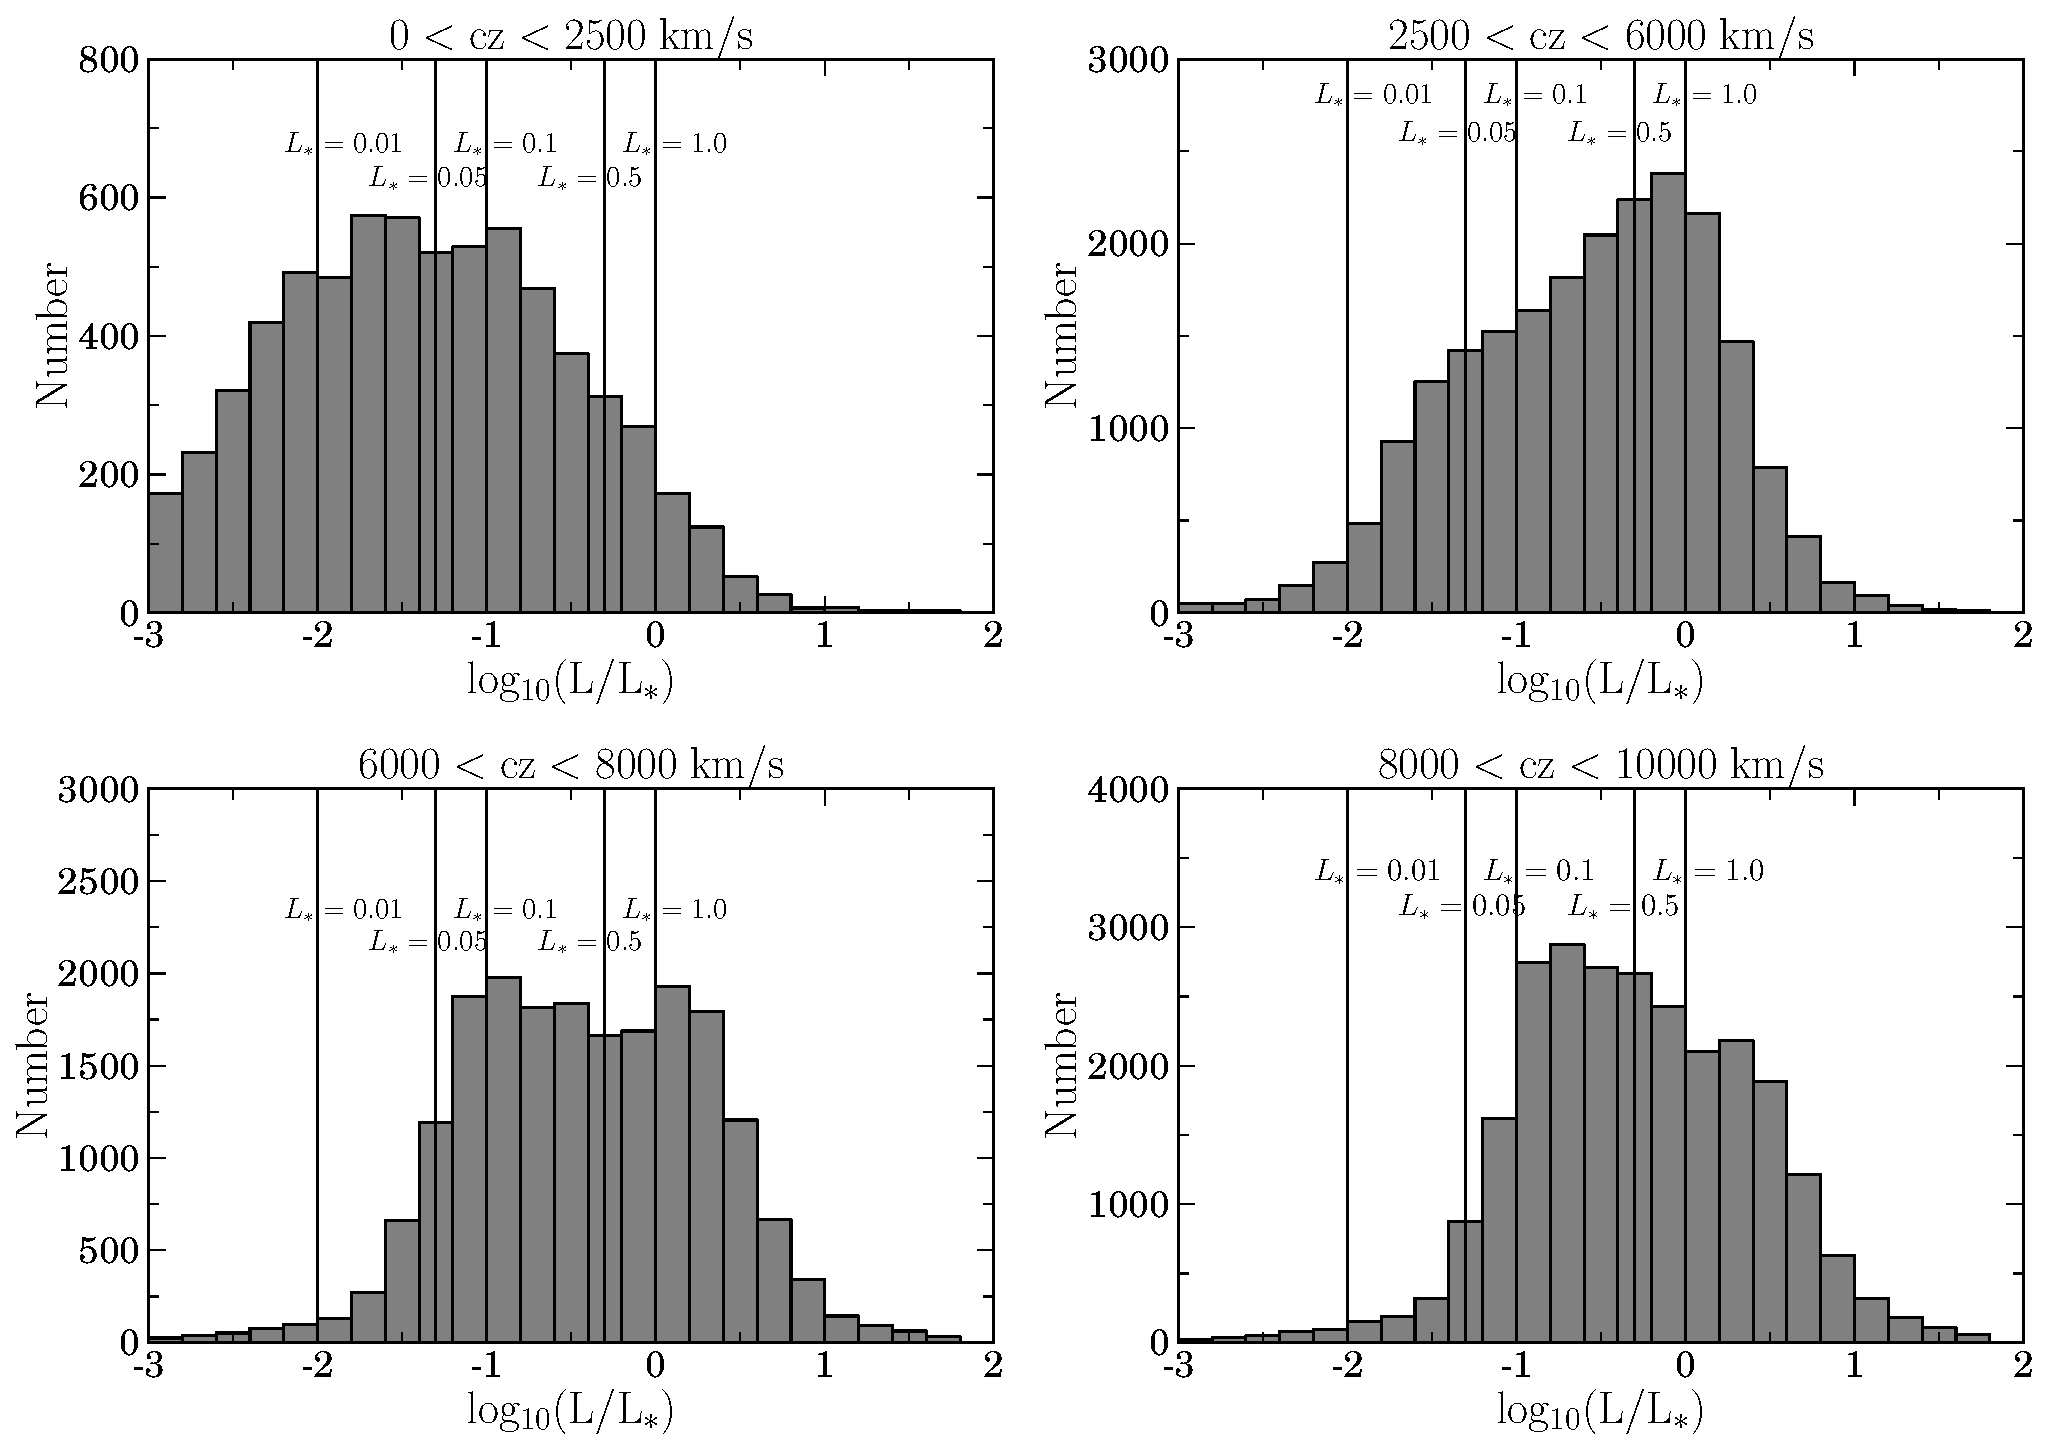
\includegraphics[width=0.50\textwidth]{Lstar_histogram_4bins_final_0-10000_v2.pdf}
        \caption{\small{Distribution of $L/L_{\**}$ values for all galaxies in the dataset. Black vertical lines highlight 1, 0.5, 0.1, 0.05 and 0.01 $L_{\**}$. The turnoff around 0.1$L_{\**}$ shows that on average, the dataset is mostly complete to 0.2$L_{\**}$.}}
%        \vspace{-5pt}
        \label{completeness}
\end{figure} 

The galaxy dataset contains over 108,000 entries, and includes data from SDSS, 2MASS, 2dF, 6dF, RC3, and many other, smaller surveys. Our criteria for including a galaxy in this dataset is only an accurate, spectroscopic redshift which places the galaxy in the $cz \leq 10,000$ km/s velocity range. This restriction leads to a completeness limit of $B \lesssim 18.7$ mag, or $\sim0.2 L_*$, at $cz = 10,000$ km/s, and progressively better towards lower velocities (see Figure \ref{completeness}). This limit will vary depending on which major surveys include a particular region of the sky. The major contributor is whether or not SDSS data is available, which begins around $cz = 5,000$ km/s. Figure \ref{completeness} is split into 4 velocity bins to illustrate this. Our data is complete down to $\sim0.1 L_*$ in the first bin, $0 \leq cz \leq 2,500$ km/s. At slightly higher velocity, $2500 \leq cz \leq 6000$ km/s, the completeness falls to barely better than $\sim1.0 L_*$ as we move past the near and well studied galaxies, but have yet to reach the footprint of deep all sky surveys. SDSS data becomes available in the last two bins, spanning $6000 \leq cz \leq 10,000$ km/s, and correspondingly completeness remains high down to the SDSS limits of $B \lesssim 18.7$ mag, or $\sim0.2 L_*$ at $cz = 10,000$ km/s.


Additionally, we have homogenized the galaxy data beyond the steps taken by NED by normalizing all measurements of galaxy inclination, position angle, and diameter to 2MASS $K$-band values. Most galaxies in NED have measures of inclination, position angle and diameter available in several different bands, so in order to make meaningful comparisons it is necessary to automatically choose one band for all measurements. We chose 2MASS values for this because it was an all-sky survey, and represents the largest fraction of available galaxy data. Physical galaxy diameters are derived from 2MASS $K_s$ ``total" angular diameter measurements and galaxy distances. 2MASS $K_s$ ``total" diameter estimates are surface brightness extrapolation measurements and are derived as 

\begin{equation}
r_{tot} = r' + a(ln(148)^b,
\end{equation}

\noindent where $r_{tot}$ is defined as the point where the surface brightness extends to 5 disk scale lengths, $r'$ is the starting point radius ($>5" - 10"$ beyond the nucleus, or core influence), and $a$ and $b$ are Sersic exponential function scale length parameters ($f = f_0 \exp{(-r/a)}^{(1/b)}$, see Jarret et al. 2003 for a full description). Approximately $50\%$ of all the galaxies have this 2MASS $K_s$ ``total" diameter. Of the remainder, $20\%$ have SDSS diameters, $27\%$ have no published diameter, and $3\%$ have diameters from other surveys. We convert values in these other bands to 2MASS $K_s$ ``total" diameters via a simple least squares linear fit when necessary.

We used $B$-band magnitudes to estimate each galaxy's luminosity in units of $L_{\**}$ as follows:

\begin{equation}
	\frac{L}{L_{\**}} = 10^{-0.4 (M_{B} - M_{B_{\**}})}.
\end{equation}

We adopt the CfA galaxy luminosity function by Marzke et al. (1994), which sets $B_{\**} $ = -19.57. Direct $B$ band measurements are available for $\sim 30\%$ of galaxies, and most of the rest have SDSS $g$ and $r$ magnitudes, which can be converted to $B$ via $B = g + 0.39 (g-r) + 0.21$ (Jester et al. 2005). Finally, we also compute an estimate of the virial radius of each galaxy as $log R_{vir} = 0.69 log D + 1.24$. This follows the parametrization of Stocke et al. (2013) relating a galaxy's luminosity to its virial radius, and the Wakker $\&$ Savage (2009) empirical relation between diameter and luminosity (see Wakker et al. 2015 and references therein for further details). Errors are propagated from the original published magnitude errors.

This homogeneous galaxy data table allows us to draw direct comparisons between the properties of the absorbers and the properties, separations, and environments of nearby galaxies with unprecedented completeness. The full dataset will be publicly released and discussed in further detail in a forthcoming paper (French et al. 2017, in prep).


\subsection{Spectra}

This initial pilot study contains 35 sightlines to bright QSOs observed with COS. We chose sightlines by first sorting the galaxy data table described above by galaxy diameter. This sorted list is then correlated with the full list of publicly available sightlines, and only those systems with impact parameter less than 500 Mpc and galaxy diameter, $D$, greater than $25$ kpc  are kept. Finally, we select the top 35 sightlines with $S/N > 11$, as sorted by galaxy diameter.

%We chose sight lines based on high S/N (generally $>$10), ease of spectral identification, and proximity to large, nearby galaxies. Several are included simply because they already have published identifications. There were no strict cutoffs for galaxy size or brightness, we simply selected the top 35 sight lines after rejecting those with lower S/N and/or more complicated features. 

All COS spectra for the target sightlines were obtained through the Barbara A. Mikulski Archive for Space Telescopes (MAST), and processed with CALCOS v3.0 or later. We combined individual exposures by the method of Wakker et al. (2015), which corrects the COS wavelength scale by cross-correlating all ISM and IGM lines in each exposure. This method addresses the up to $\pm40$ km/s misalignments produced by CALCOS, and produces a corrected error array based on Poisson noise, which better matches the measured errors than the errors delivered in the x1d files. We then combine multiple exposures by aligning Galactic absorption lines with 21-cm spectra, and adding up the total counts in each pixel before converting to flux using the original, average flux-count ratio at each wavelength.

\begin{figure}[ht!]
\centering
  \subfigure[]{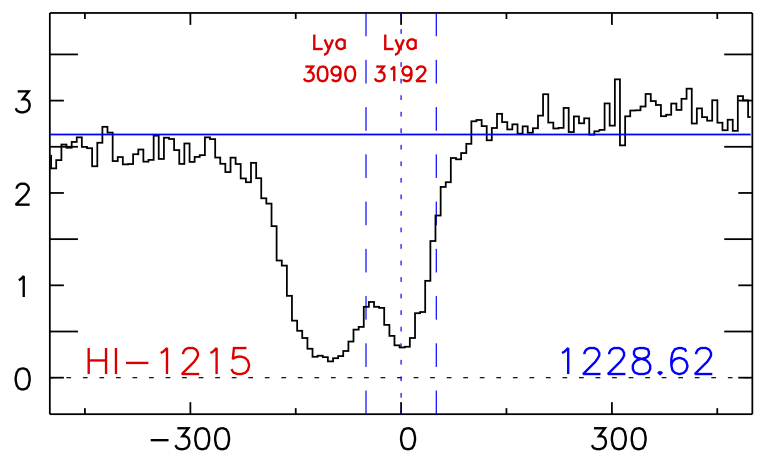
\includegraphics[width=0.95\linewidth]{MRK290_system-3192_cut.jpg}}{\label{line}}
  \subfigure[]{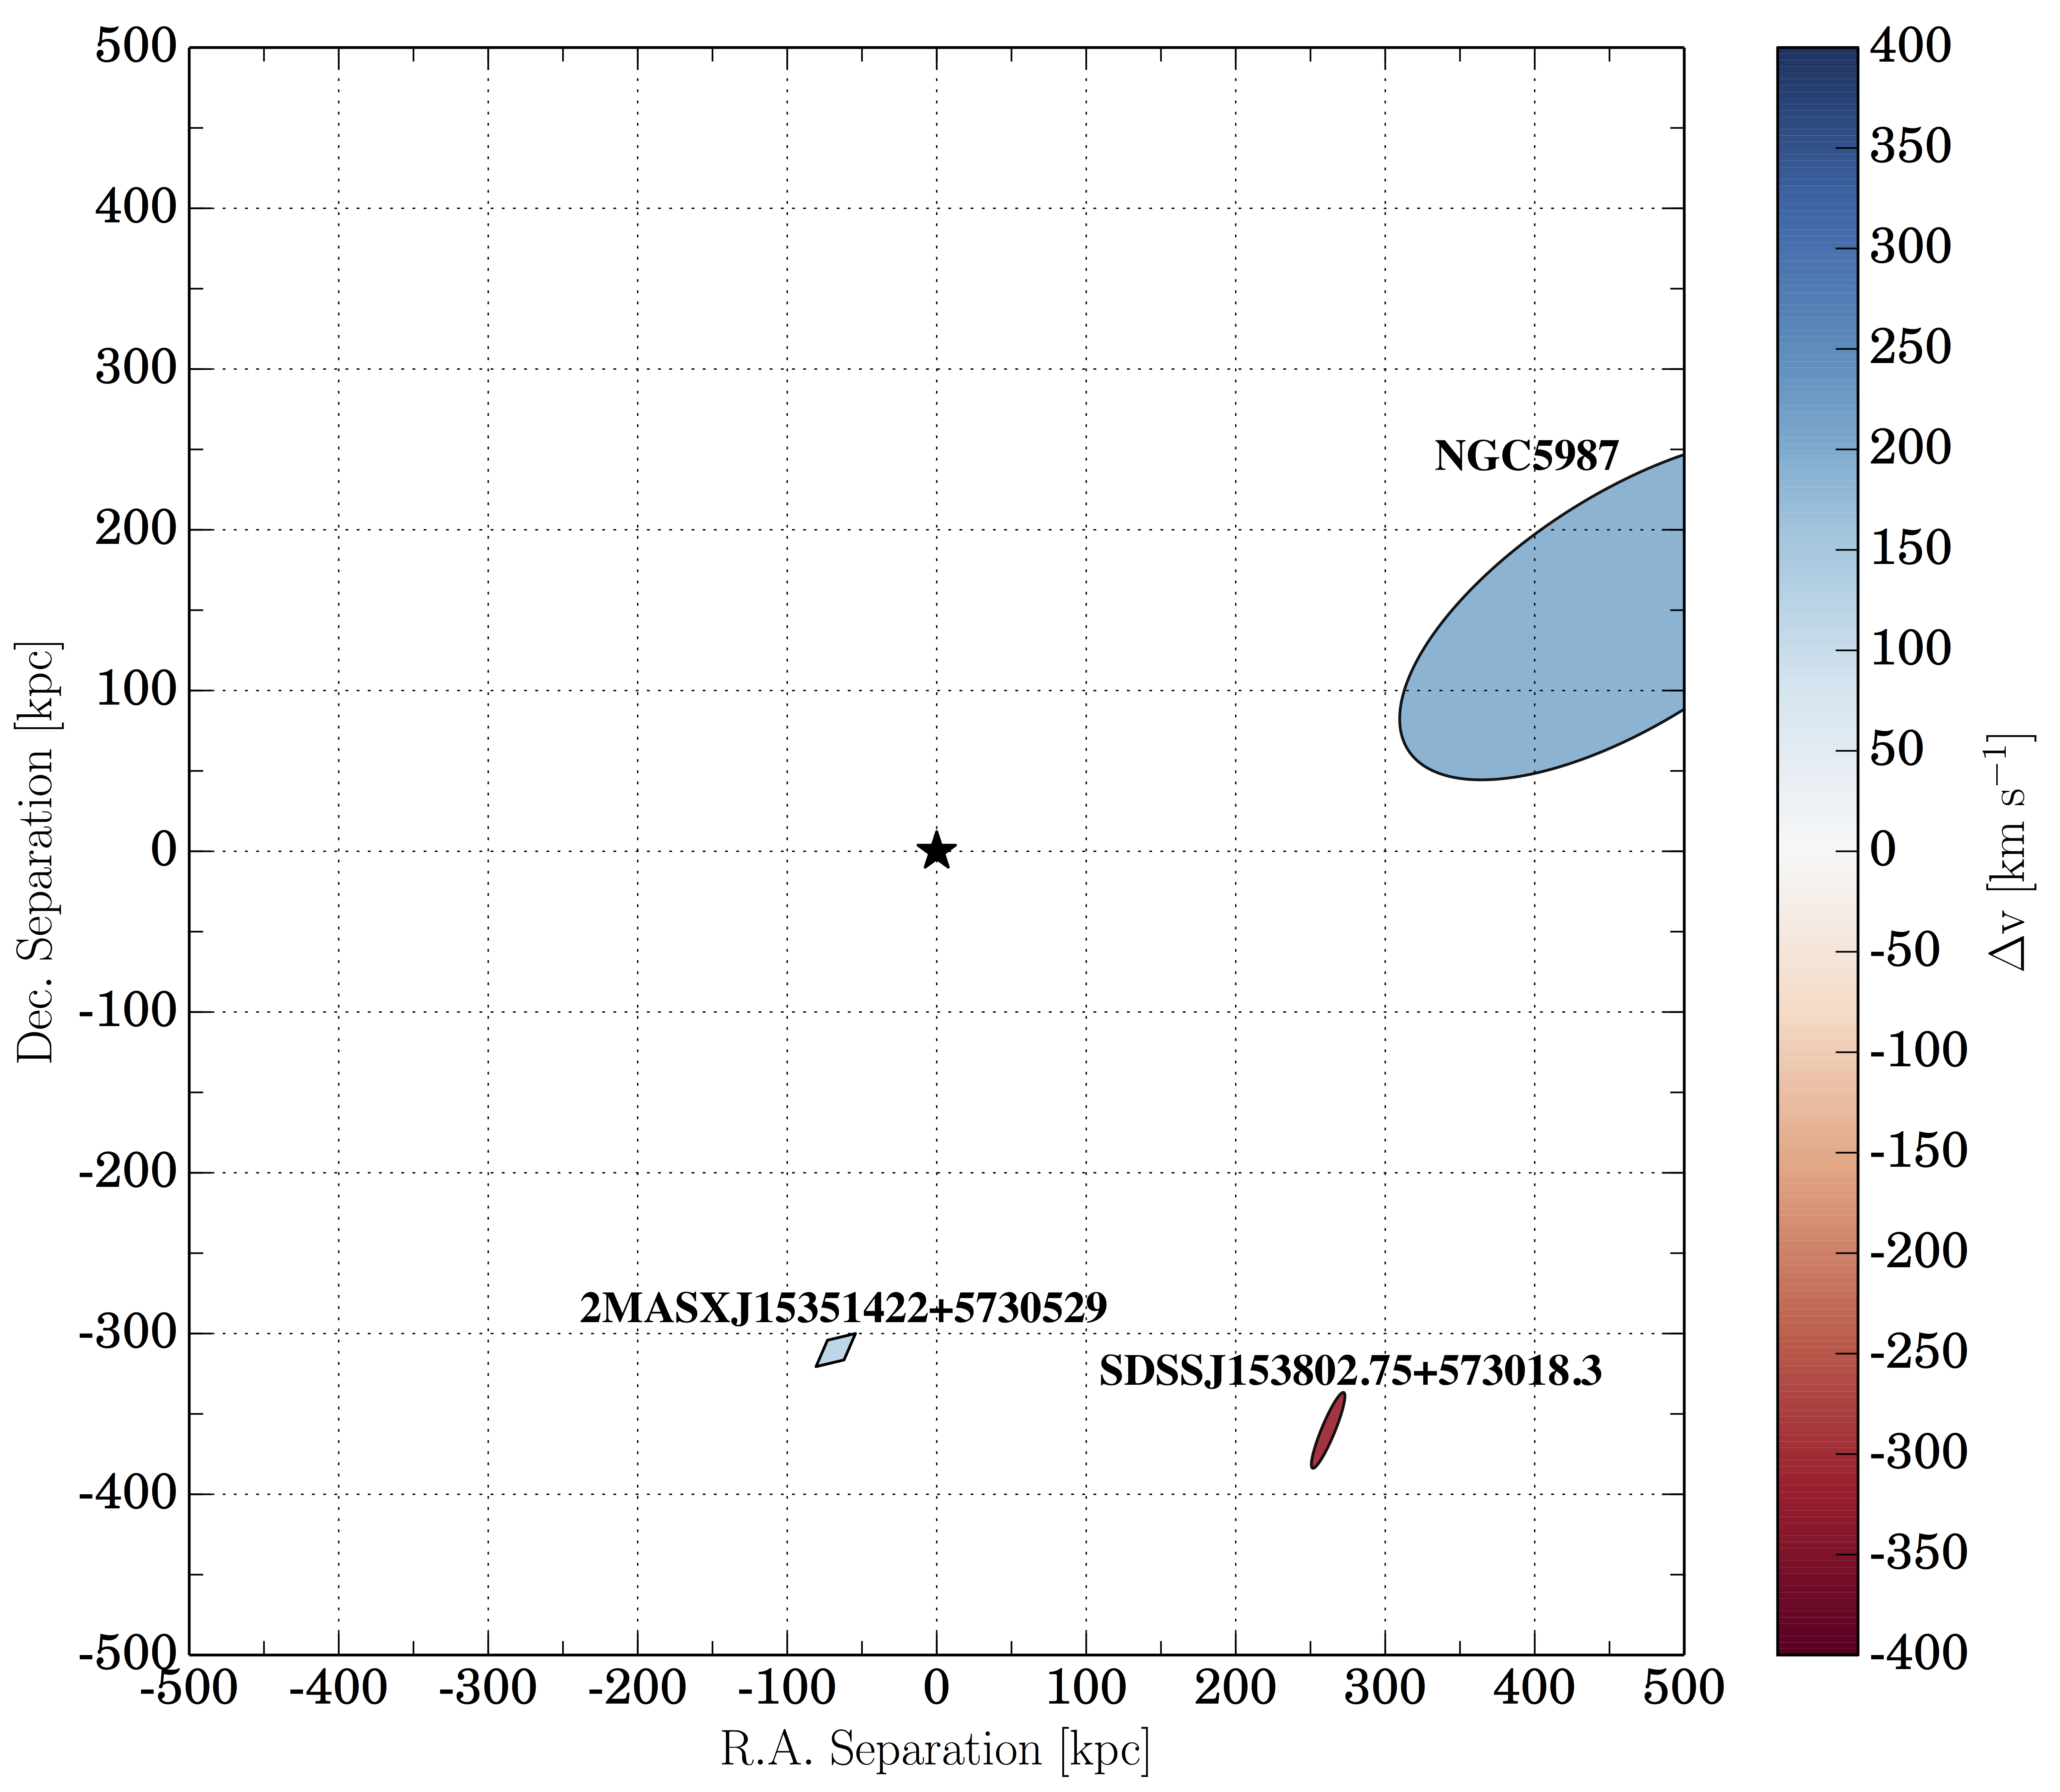
\includegraphics[width=1.\linewidth]{map_MRK290_3207_v2.jpg}\label{impactmap}}
  \caption{\small{a) An example of Ly$\alpha$ lines found in a sightline towards MRK290 at 3090 and 3192 km/s. b) A map of \textit{all} galaxies within a 500 kpc impact parameter of target MRK290 sightline and with velocity ($cz$) within 400 km/s of absorption detected at 3090 and 3192 km/s (central black star). The galaxy NGC5987 ($v=3010$ km/s, inclination = $65^{\circ}$) can be unambiguously paired with the Ly$\alpha$ absorption features at $v=3090, 3192$ km/s because it is the largest and closest galaxy in both physical and velocity space to the absorption feature.}}
\vspace{5pt}
\end{figure}

%The STIS data was processed in the same manner as described in Wakker $\&$ Savage (2009), and thus we only give a short summary here. The STIS calibrated fits files were downloaded from MAST, and STIS-E140M echelle orders were combined into a single spectrum. The photon counts and errors were interpolated onto a common grid, counts were added and weighted by the rms at each pixel, and finally converted back to flux. Table \ref{target_table} summarizes the properties of the selected QSO targets.


\begin{table*}[ht]\footnotesize
\begin{center}
\begin{tabular}{l l l c c c c c c c c c c c c}
 \hline \hline
  Target & Galaxy & $\mathcal{L}$ & $R_{vir}$ & $\rho$ (kpc) & $v_{galaxy}$ & $\Delta v$  &  Inc.   &  Az.     & $v_{Ly\alpha}$ & $$W$_{Ly\alpha}$ \\ 
  	     &               &                      & \scriptsize [kpc] & \scriptsize [kpc] & \scriptsize [km/s] & \scriptsize [km/s] & \scriptsize [deg] & \scriptsize [deg] & \scriptsize [km/s] & \scriptsize [m\AA]	\\
 \scriptsize (1) & \scriptsize (2) & \scriptsize (3) & \scriptsize (4) & \scriptsize (5) & \scriptsize (6) & \scriptsize  (7) & \scriptsize (8) & \scriptsize (9) & \scriptsize (10) & \scriptsize (11) \\ \hline \hline

1H0717+714  &  UGC03804  &  0.24  &  173  &  207  &  2887  &  17  &  53  &  7  &  2870  &  343$\pm$6  \\
1H0717+714  &  UGC03804  &  0.21  &  173  &  207  &  2887  &  -69  &  53  &  7  &  2956  &  39$\pm$4  \\
2dFGRS\_S393Z082  &  NGC1097  &  1.8*  &  273  &  112  &  1271  &  32  &  47  &  12  &  1239  &  570$\pm$21  \\
3C66A  &  UGC01832  &  1.7  &  192  &  56  &  5913  &  -52  &  65  &  16  &  5965  &  53$\pm$6  \\
FBQSJ1431+2442  &  IRASF14291+2443  &  0.074*  &  203  &  328  &  6615  &  73  &  74  &  x  &  6542  &  56$\pm$15  \\
FBQSJ1431+2442  &  IRASF14291+2443  &  0.085*  &  203  &  328  &  6615  &  -8  &  74  &  x  &  6623  &  272$\pm$20  \\
H1101-232  &  MCG-04-26-019  &  0.33  &  173  &  179  &  3623  &  43  &  65  &  26  &  3580  &  573$\pm$12  \\
HE0241-3043  &  NGC1097  &  1.4*  &  273  &  219  &  1271  &  50  &  47  &  62  &  1221  &  83$\pm$12  \\
HE0241-3043  &  NGC1097  &  1.4*  &  273  &  219  &  1271  &  -39  &  47  &  62  &  1310  &  184$\pm$15  \\
LBQS1230-0015  &  NGC4517  &  1.4  &  193  &  110  &  1128  &  1  &  83  &  90  &  1127  &  473$\pm$16  \\
MRC2251-178  &  MCG-03-58-009  &  1.4*  &  319  &  320  &  9030  &  -21  &  59  &  39  &  9051  &  60$\pm$4  \\
MRK1014  &  NGC0768  &  0.12*  &  253  &  486  &  7021  &  -59  &  73  &  85  &  7080  &  117$\pm$11  \\
MRK290  &  NGC5987  &  0.77*  &  322  &  486  &  3010  &  -95  &  65  &  12  &  3105  &  511$\pm$5  \\
MRK290  &  NGC5987  &  0.37*  &  322  &  486  &  3010  &  -197  &  65  &  12  &  3207  &  319$\pm$4  \\
MRK876  &  UGC10294  &  0.063  &  165  &  274  &  3504  &  26  &  50  &  7  &  3478  &  280$\pm$3  \\
PG0003+158  &  NGC7814  &  0.081  &  171  &  197  &  1050  &  217  &  65  &  47  &  833  &  131$\pm$15  \\
PG0832+251  &  KUG0833+252  &  0.041  &  165  &  294  &  6964  &  -16  &  60  &  55  &  6980  &  133$\pm$14  \\
PG0832+251  &  KUG0833+252  &  0.01  &  165  &  294  &  6964  &  -237  &  60  &  55  &  7201  &  48$\pm$10  \\
PG1001+054  &  UGC05432  &  0.14  &  164  &  217  &  3995  &  -97  &  35  &  78  &  4092  &  222$\pm$10  \\
PG1302-102  &  NGC4939  &  0.05*  &  235  &  265  &  3110  &  -338  &  46  &  61  &  3448  &  71$\pm$5  \\
RBS1768  &  RFGC3781  &  0.056*  &  253  &  464  &  9162  &  -198  &  81  &  x  &  9360  &  364$\pm$4  \\
RBS1768  &  RFGC3781  &  0.024*  &  253  &  464  &  9162  &  -272  &  81  &  x  &  9434  &  160$\pm$5  \\
RX\_J0714.5+7408  &  UGC03717  &  0.13*  &  202  &  271  &  4188  &  114  &  61  &  83  &  4074  &  58$\pm$7  \\
RX\_J0714.5+7408  &  UGC03717  &  0.15*  &  202  &  271  &  4188  &  -76  &  61  &  83  &  4264  &  410$\pm$9  \\
RX\_J1017.5+4702  &  NGC3198  &  0.02  &  191  &  378  &  663  &  34  &  70  &  55  &  629  &  60$\pm$17  \\
RX\_J1117.6+5301  &  NGC3631  &  0.32  &  187  &  198  &  1156  &  25  &  16  &  x  &  1131  &  356$\pm$20  \\
RX\_J1117.6+5301  &  NGC3631  &  0.25  &  187  &  198  &  1156  &  -103  &  16  &  x  &  1259  &  57$\pm$17  \\
RX\_J1236.0+2641  &  NGC4565  &  0.54*  &  292  &  159  &  1230  &  218  &  83  &  39  &  1012  &  337$\pm$32  \\
RX\_J1236.0+2641  &  NGC4565  &  1.7*  &  292  &  159  &  1230  &  42  &  83  &  39  &  1188  &  288$\pm$24  \\
RX\_J1236.0+2641  &  NGC4559  &  0.27  &  165  &  188  &  807  &  12  &  62  &  31  &  795  &  295$\pm$37  \\
RX\_J1330.8+3119  &  UGC08492  &  0.081*  &  204  &  335  &  7414  &  13  &  16  &  41  &  7401  &  330$\pm$15  \\
RX\_J1356.4+2515  &  CGCG132-055  &  0.35*  &  206  &  190  &  8671  &  196  &  35  &  25  &  8475  &  126$\pm$18  \\
RX\_J1503.2+6810  &  CGCG318-012  &  0.031*  &  250  &  325  &  9765  &  -357  &  50  &  1  &  10122  &  44$\pm$14  \\
RX\_J1544.5+2827  &  CGCG166-047  &  0.031  &  175  &  326  &  9646  &  4  &  42  &  61  &  9642  &  183$\pm$14  \\
RX\_J1544.5+2827  &  CGCG166-047  &  0.023  &  175  &  326  &  9646  &  -113  &  42  &  61  &  9759  &  169$\pm$12  \\
RX\_J2043.1+0324  &  NGC6954  &  0.037  &  166  &  301  &  4067  &  -13  &  55  &  66  &  4080  &  82$\pm$10  \\
RX\_J2139.7+0246  &  UGC11785  &  1.5  &  203  &  108  &  4074  &  -9  &  80  &  69  &  4083  &  490$\pm$7  \\
RX\_J2139.7+0246  &  UGC11785  &  1.2*  &  203  &  108  &  4074  &  -107  &  80  &  69  &  4181  &  529$\pm$7  \\
SBS0957+599  &  MCG+10-14-058  &  1.4*  &  261  &  206  &  9501  &  32  &  71  &  19  &  9469  &  78$\pm$12  \\
SDSSJ021218.32-073719.8  &  SDSSJ021315.79-073942.7  &  0.09  &  174  &  268  &  4800  &  44  &  50  &  10  &  4756  &  528$\pm$15  \\
SDSSJ021218.32-073719.8  &  SDSSJ021315.79-073942.7  &  0.092  &  174  &  268  &  4800  &  -33  &  50  &  10  &  4833  &  500$\pm$17  \\
SDSSJ080838.80+051440.0  &  UGC04239  &  0.87*  &  279  &  378  &  8763  &  23  &  44  &  38  &  8740  &  883$\pm$24  \\
SDSSJ080838.80+051440.0  &  UGC04239  &  0.45*  &  279  &  378  &  8763  &  -164  &  44  &  38  &  8927  &  130$\pm$19  \\
SDSSJ091728.60+271951.0  &  UGC04895  &  0.022*  &  204  &  408  &  7073  &  -68  &  59  &  32  &  7141  &  374$\pm$23  \\
SDSSJ112224.10+031802.0  &  NGC3640  &  0.4  &  180  &  139  &  1251  &  202  &  37  &  22  &  1049  &  288$\pm$30  \\
SDSSJ112224.10+031802.0  &  NGC3640  &  1.1  &  180  &  139  &  1251  &  -13  &  37  &  22  &  1264  &  424$\pm$27  \\
SDSSJ130524.30+035731.0  &  UGC08186  &  1.3*  &  268  &  249  &  7006  &  -33  &  76  &  14  &  7039  &  480$\pm$14  \\
SDSSJ135726.27+043541.4  &  NGC5364  &  0.74*  &  211  &  183  &  1241  &  117  &  55  &  84  &  1124  &  85$\pm$11  \\
SDSSJ135726.27+043541.4  &  NGC5364  &  0.97*  &  211  &  183  &  1241  &  -55  &  55  &  84  &  1296  &  98$\pm$9  \\
SDSSJ140428.30+335342.0  &  KUG1402+341  &  1.4  &  204  &  118  &  7919  &  35  &  69  &  63  &  7884  &  889$\pm$28  \\
TON1009  &  NGC2770  &  0.19*  &  204  &  274  &  1947  &  -14  &  78  &  43  &  1961  &  350$\pm$21  \\
 \\
\hline
\end{tabular}
\end{center}
  \caption{\small{All associated systems. The largest $\mathcal{L}$ value is given, where a (\**) indicates $d^{1.5}$ was used, otherwise the quoted $\mathcal{L}$ was computed with $R_{vir}$. For all entries, 'x' indicates unknown values.}}
  \label{target_table}
\end{table*}


%\begin{figure*}[ht!]
%  \centering
%  \subfigure[]{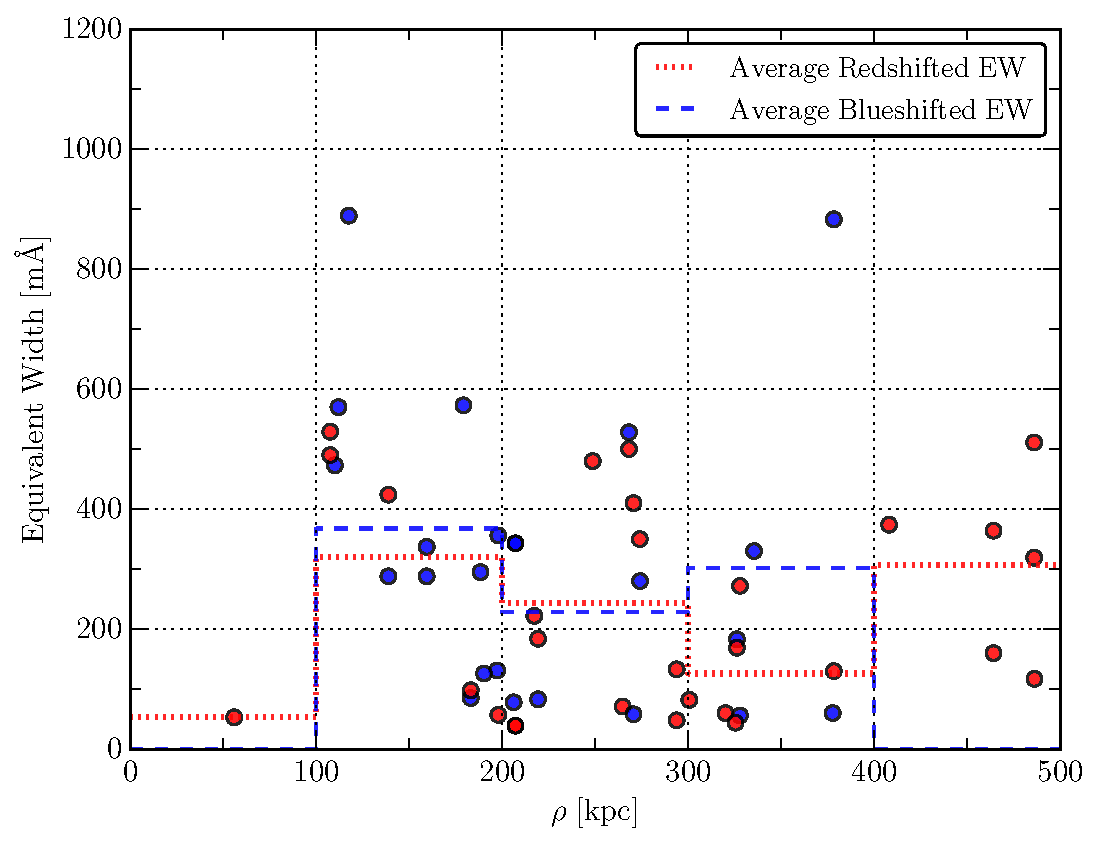
\includegraphics[scale=0.48]{W(impact)_avgHistograms.pdf}}{\label{ew_vs_impact}}\vspace{-5pt}
%  \subfigure[]{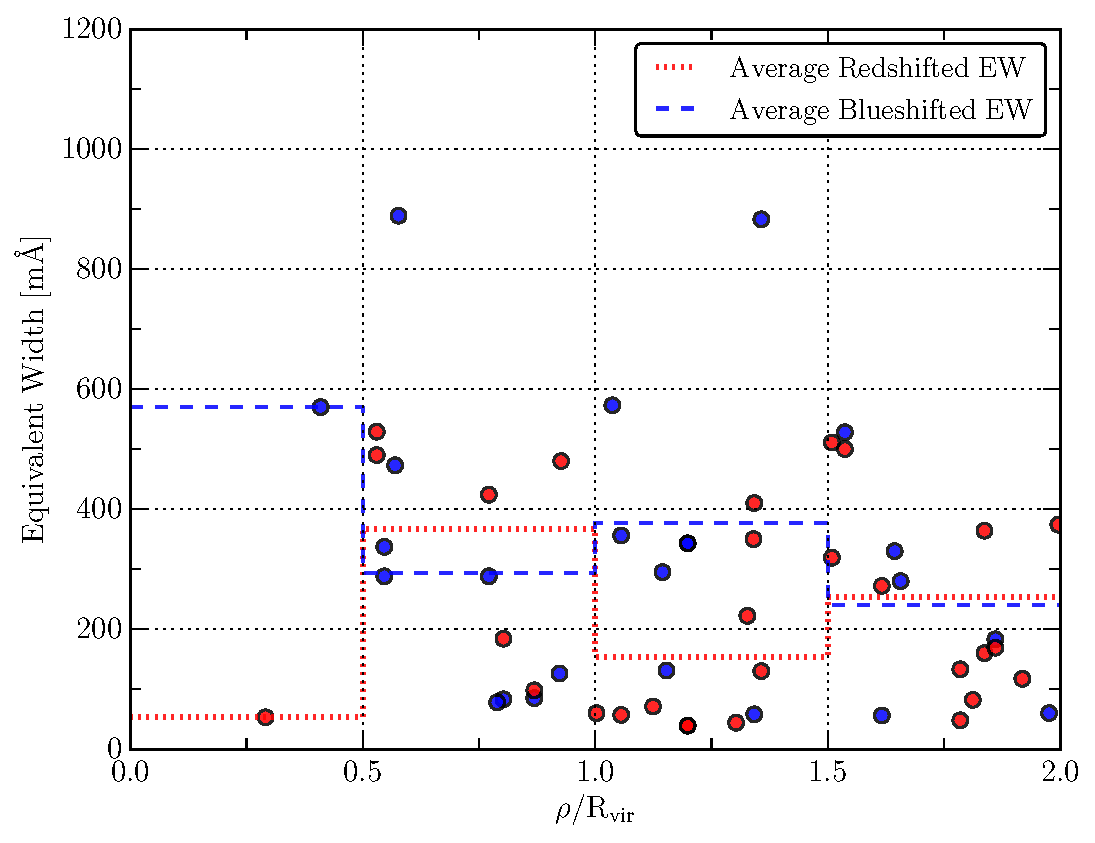
\includegraphics[scale=0.48]{W(impact_vir)_avgHistograms.pdf}}{\label{ew_vs_impact-d}}
%  \caption{\small{a) Equivalent width ($EW$) of each absorber as a function of $\rho$ (kpc), b) ($EW$) as a function of $\rho/R_{vir}$. The anti-correlation is strongest when scaling $\rho$ by the galaxy virial radius.}}
%  \vspace{10pt}
% \label{ew_both}
%\end{figure*}


\section{Results}

We have identified 51 Ly$\alpha$ absorption lines in the spectra of our initial 35 QSO sample which can be unambiguously associated with a single nearby galaxy of diameter $D\geq25$ kpc. In order to be considered for a pairing, a galaxy and absorption feature must appear within 400 km/s in velocity and 500 kpc in physical impact parameter from each other. When multiple galaxies pass these criteria for a particular line, we are left with two options. 1) one galaxy is obviously far larger and closer in physical and velocity space to the line, and may have several satellite galaxies, or 2) no single galaxy if obviously dominant, and we do not include this line in further analysis. 

\begin{figure*}[t]
\centering
\subfigure[]{\label{ew_vs_impact}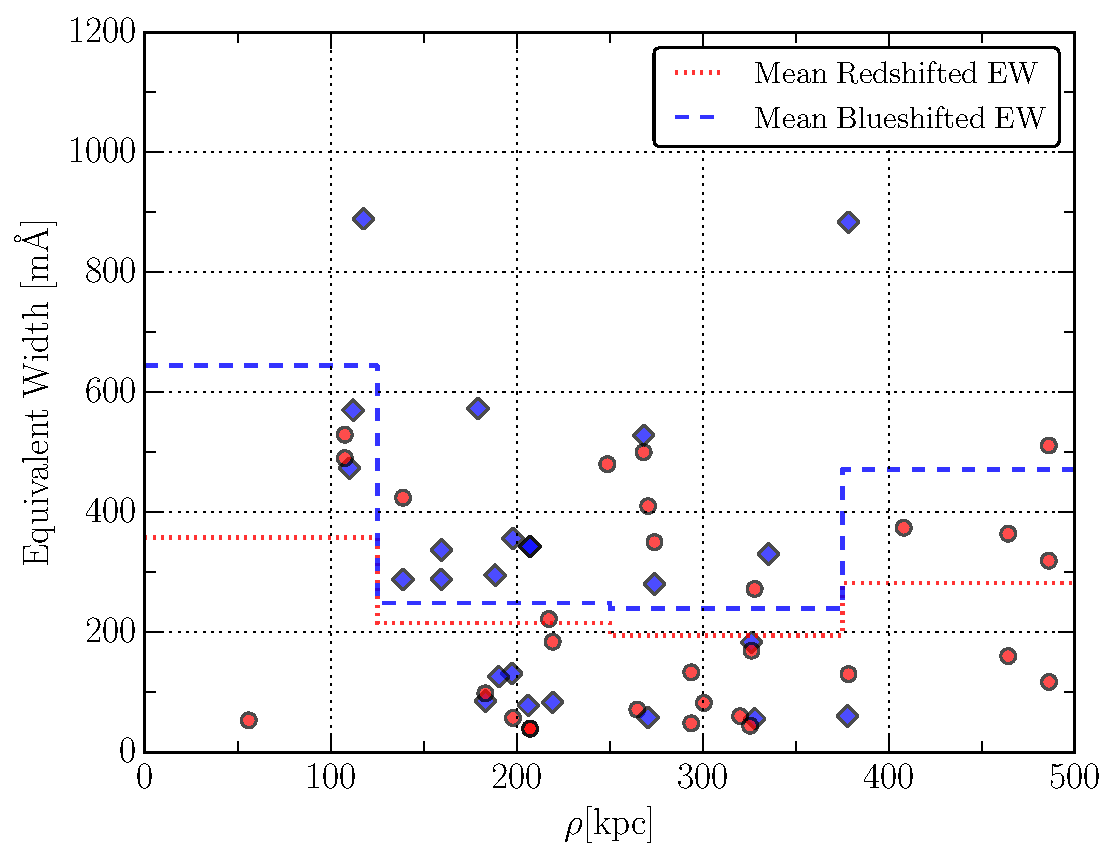
\includegraphics[width=0.49\textwidth]{W(impact)_mean_125_difHistograms.pdf}}
\subfigure[]{\label{ew_vs_impact_vir}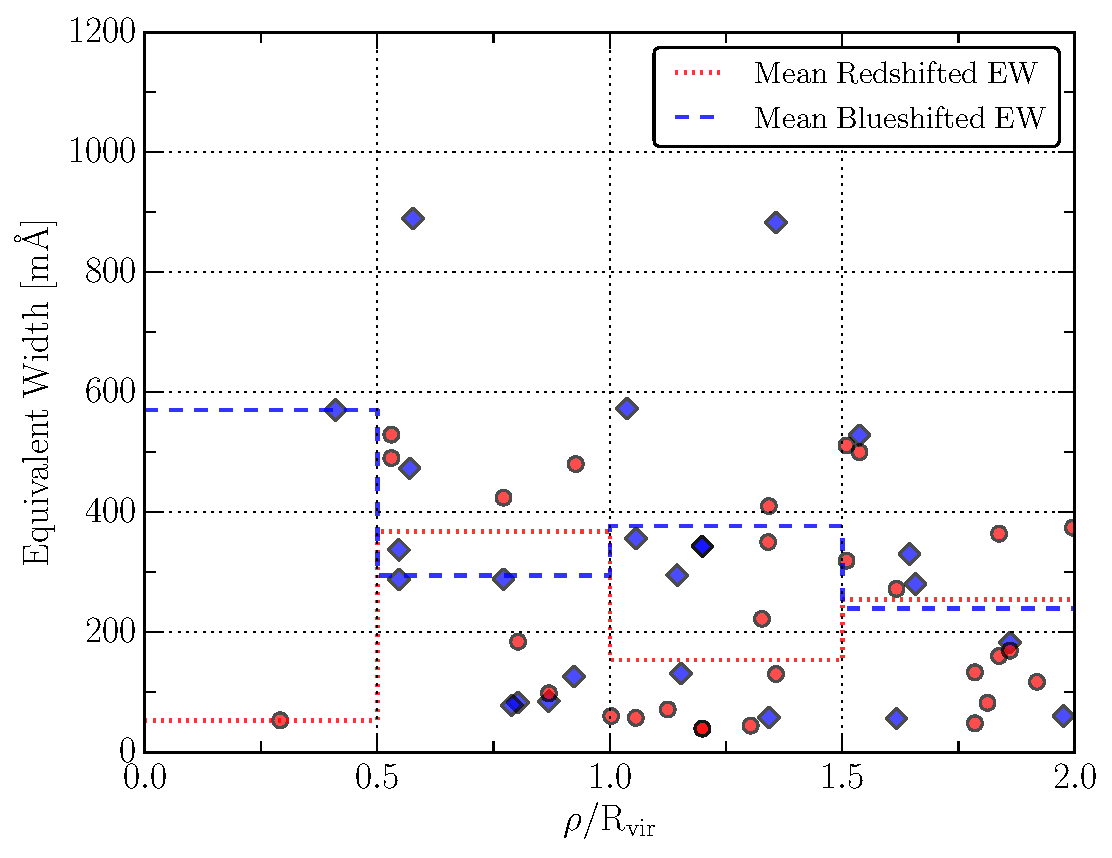
\includegraphics[width=0.49\textwidth]{W(impact_vir)_mean_0p5_difHistograms.pdf}}
\caption{\small{a) Equivalent width of each absorber as a function of impact parameter, $\rho$ (kpc), b) Equivalent width as a function of $\rho/R_{vir}$. The anti-correlation is strongest when scaling $\rho$ by the galaxy virial radius. Absorbers are separated into red and blue-shifted samples based on $\Delta v$. Bins of mean $EW$ are overplotted in red-dashed, and blue-dotted lines for their respective samples.}}
\vspace{5pt}
\end{figure*}


To facilitate this decision, we calculate the likelihood, $\mathcal{L}$, of every possible galaxy-absorber pairing as follows:

\begin{equation}
	\mathcal{L} = A e^{-(\frac{\rho}{R_{eff}})^2} e^{-(\frac{\Delta v}{200})^2}.
\end{equation}


\noindent Here $\rho$ is the physical impact parameter, $\Delta v$ the velocity difference between the absorber and the galaxy ($\Delta v = v_{galaxy} - v_{absorber}$), and $A$ is a factor included to increase the likelihood in the case that $R_{eff} \geq \rho$ (in which case $A = 2$, otherwise $A = 1$). We compute $\mathcal{L}$ for two different values of $R_{eff}$: $R_{vir}$, the virial radius of the galaxy, and $d^{1.5}$, the major diameter of the galaxy to the power of 1.5. $\mathcal{L}$ computed with $R_{vir}$ is liable to select satellite galaxies instead of the larger hosts, so including a version with $d^{1.5}$ serves as a two-tiered selection system. An absorber-galaxy system separated by 200 km/s in velocity and 1$R_{vir}$ would have $\mathcal{L} = 0.27$. In order for an absorber to be marked as ``associated" with a particular galaxy, we require that its $\mathcal{L}$ must be a factor of 5 larger than the next best possible association, and $\mathcal{L} \ge 0.01$ for at least one of $\mathcal{L}_{R_{vir}}$ or $\mathcal{L}_{D^{1.5}}$. We visually inspect systems with only one $\mathcal{L}$ meeting these criteria, and decide to reject or include it based on the complexity of the nearby galaxy environment. 

Figures \ref{line} and \ref{impactmap} show a clean example of a Ly$\alpha$ absorption line with a map of its galaxy environment, showing an unambiguous pairing between the absorption features at $3090, 3192$ km/s toward MRK290 and galaxy NGC5987 ($\mathcal{L} = 0.37$). Unless explicitly stated, all following analysis concerns similarly unambiguous ``associated" systems. 

Additionally, we split the absorber-galaxy catalog based on the velocity difference of the two, $\Delta v$. With this scheme, we refer to an absorber with a velocity \textit{lower} than the associated galaxy as \textit{blueshifted}, while an absorber with a velocity \textit{higher} is referred to as \textit{redshifted}. The rest of the results will be analyzed based upon this splitting. 


\begin{figure*}[ht]
\centering
\subfigure[]{\label{w_vir}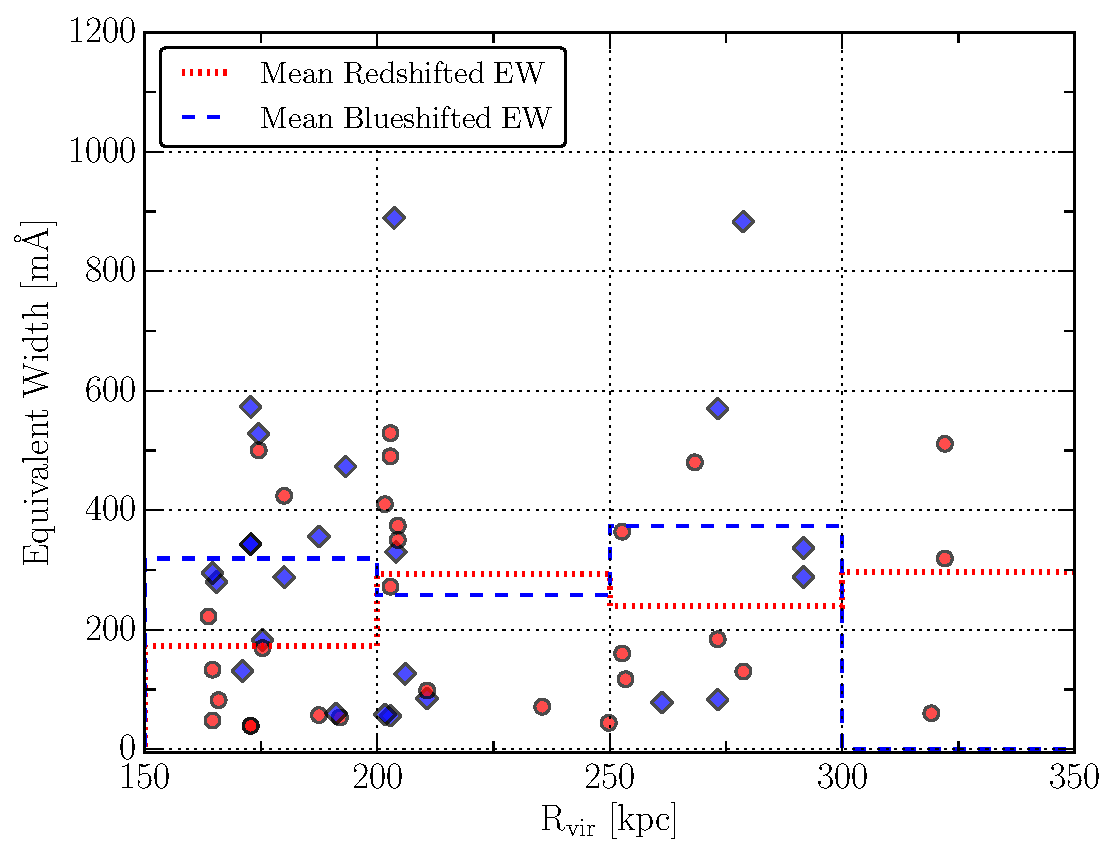
\includegraphics[width=0.48\textwidth]{W(vir)_avgHistograms.pdf}}
\subfigure[]{\label{impact_vir}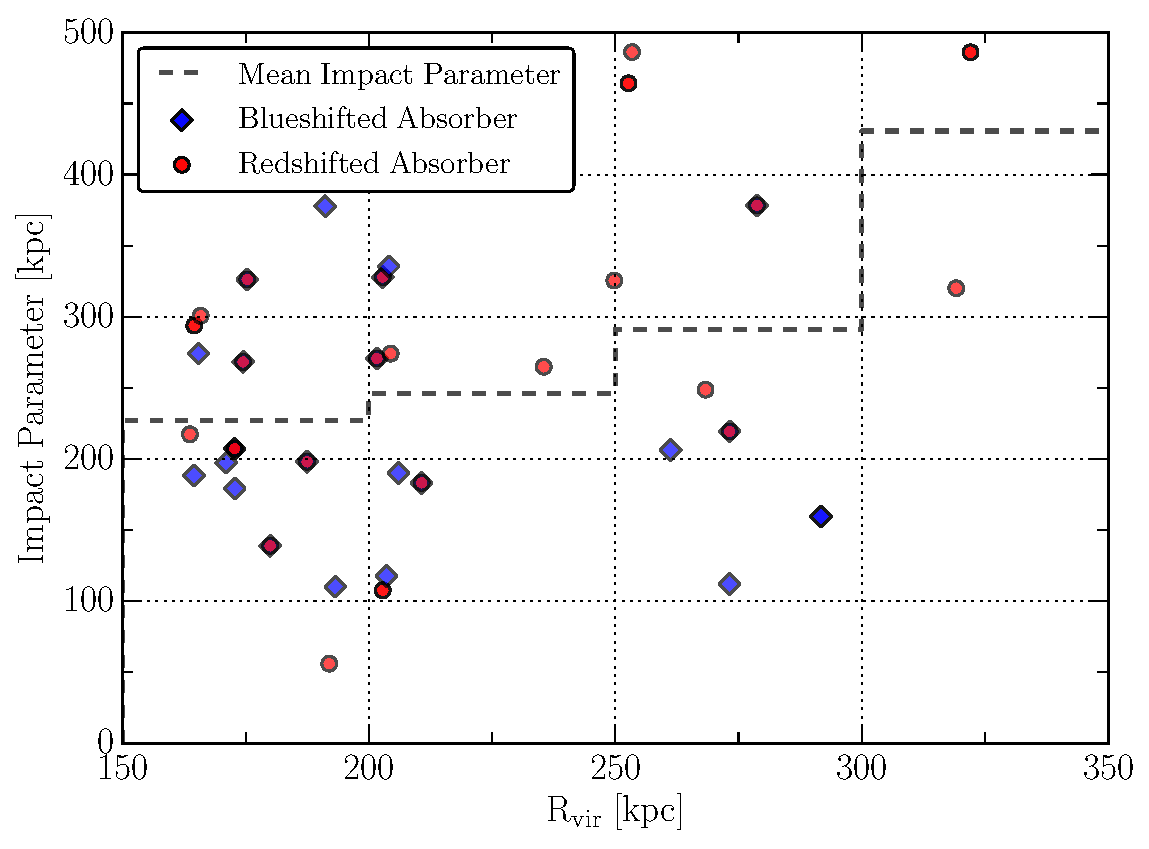
\includegraphics[width=0.48\textwidth]{impact(virial)_mean_50_Histograms.pdf}}
\caption{\small{a) Equivalent width of each absorber as a function of the virial radius of the associated galaxy. The blue-dotted and red-dashed lines shows the average $EW$ in 50 kpc bins of impact parameter for the blueshifted and redshifted absorbers, respectively. b) Impact parameter to each absorber as a function of the virial radius of the associated galaxy. The blue-dotted and red-dashed lines shows the average impact parameter in 50 kpc bins of $R_{vir}$ for the blueshifted and redshifted absorbers, respectively.}}
\vspace{5pt}
\end{figure*}


%For all distributions, we employ and quote the results of both the Kolmogorov-Smirnov (KS) and the Anderson-Darling (AD) statistical tests.


%\begin{figure}[h!]
%        \centering
%        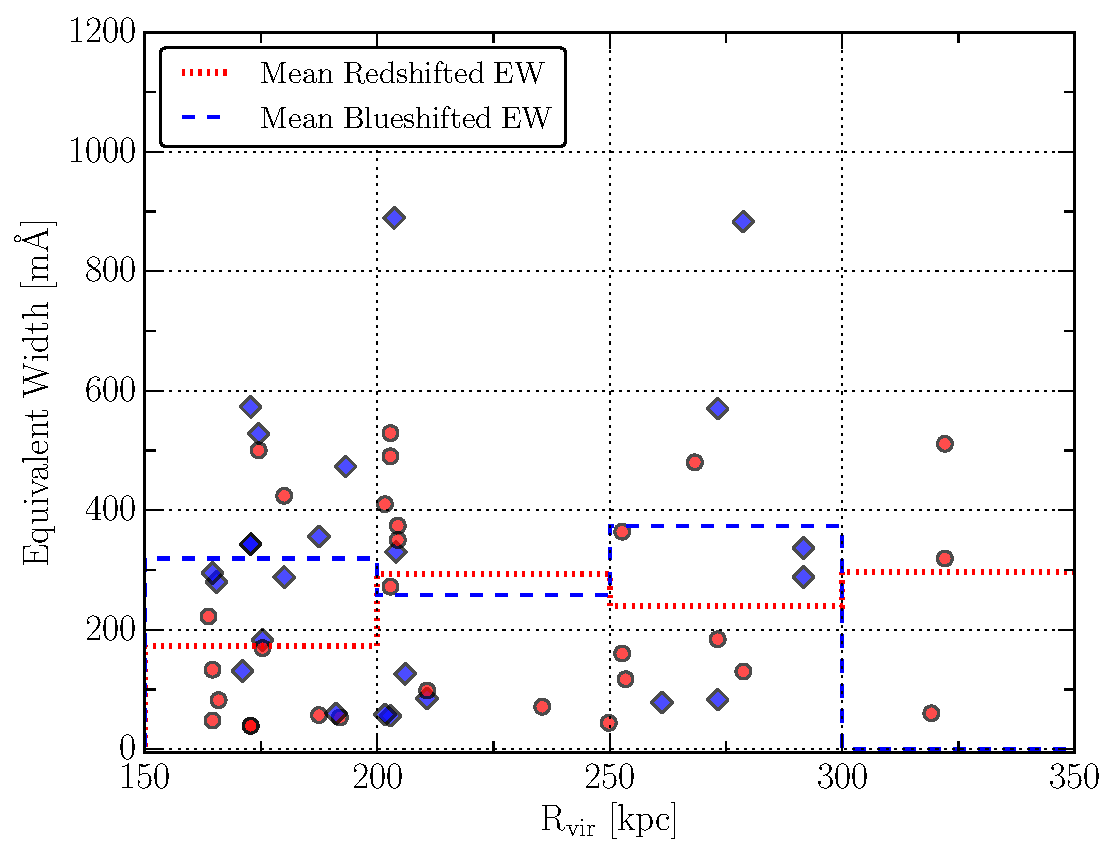
\includegraphics[width=0.48\textwidth]{W(vir)_avgHistograms.pdf}
%        \caption{\small{Equivalent width of each absorber as a function of the virial radius of the associated galaxy in the sample. The blue-dotted and red-dashed lines shows the average $EW$ in 50 kpc bins of impact parameter for the blueshifted and redshifted absorbers, respectively.}}
%        \label{w_vir}
%        \vspace{5pt}
%\end{figure}
%
%\begin{figure}[h!]
%        \centering
%        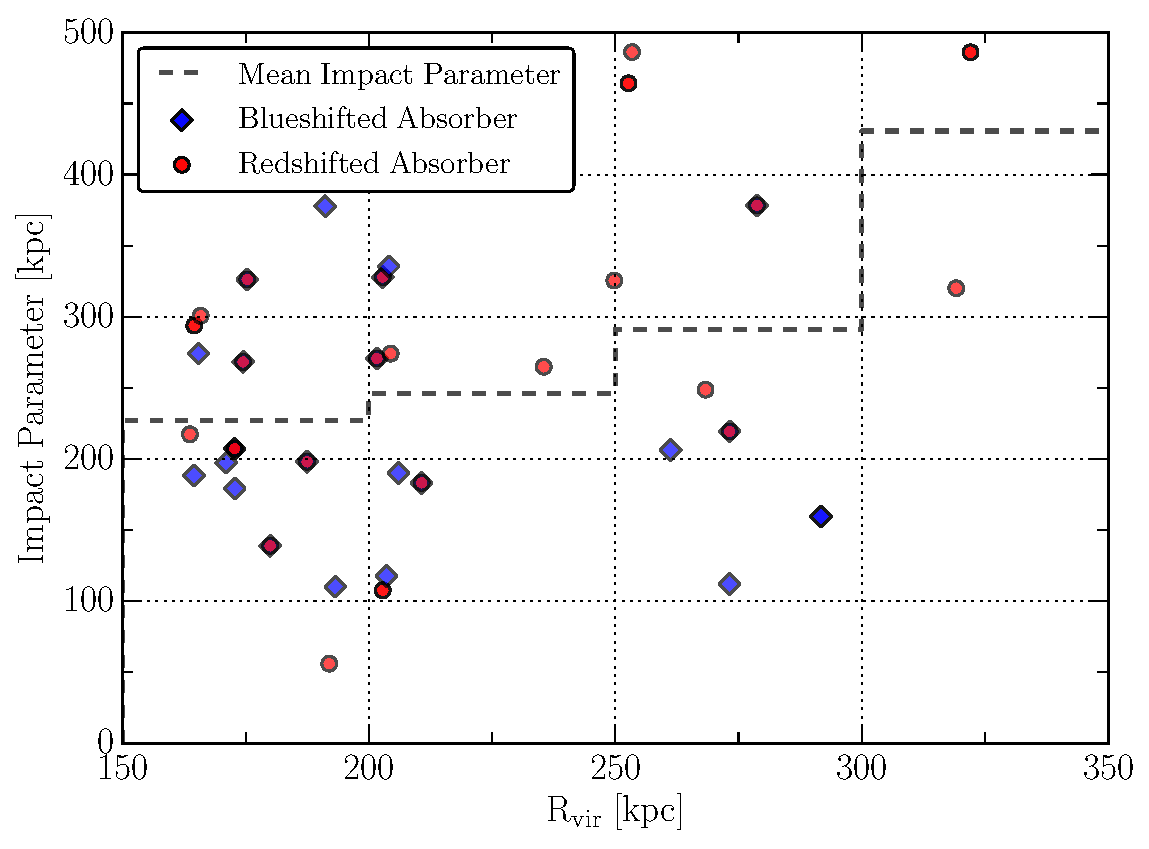
\includegraphics[width=0.48\textwidth]{impact(virial)_mean_50_Histograms.pdf}
%        \caption{\small{Impact parameter to each absorber as a function of the virial radius of the associated galaxy in the sample. The blue-dotted and red-dashed lines shows the average impact parameter in 50 kpc bins of $R_{vir}$ for the blueshifted and redshifted absorbers, respectively.}}
%        \label{w_vir}
%        \vspace{5pt}
%\end{figure}


\vspace{10pt}


\subsection{EW-$\rho$ Anti-correlation}
Numerous previous studies have suggested that Ly$\alpha$ equivalent width ($EW$) is anti-correlated with impact parameter ($\rho$) to the nearest galaxy. We find a weak correlation, as shown in Figure \ref{ew_vs_impact}. However, we find a stronger anti-correlation when we normalize $\rho$ by $R_{vir}$. Figure \ref{ew_vs_impact_vir} shows this expected anti-correlation when plotting $EW$ vs $\rho/R_{vir}$. A possible explanation for this trend is that larger galaxies host larger, more physically extended CGM halos. We would thus expect the absorber $EW$ to also correlate positively with $R_{vir}$. Figure \ref{w_vir} shows $EW$ as a function of $R_{vir}$, with the blue-dashed and red-dotted lines show the average $EW$ in bins of 50 kpc of $R_{vir}$, showing little evidence of a correlation. However, by similary plotting $\rho$ as a function of $R_{vir}$, we instead find some evidence that absorbers around larger galaxies tend to be found at higher impact parameters. While we expect the upper-left quadrant of this figure to be sparsely populated (our likelihood-based method would tend not to choose small galaxies at large distances), it is unclear to us why the lower-right quadrant (large galaxies with absorbers at low impact parameter) is also sparsely populated. The full-sized sample at the completion of our study should provide a clearer picture.


%\begin{figure*}[h!]
%\centering
%\begin{minipage}[b]{.49\textwidth}
%        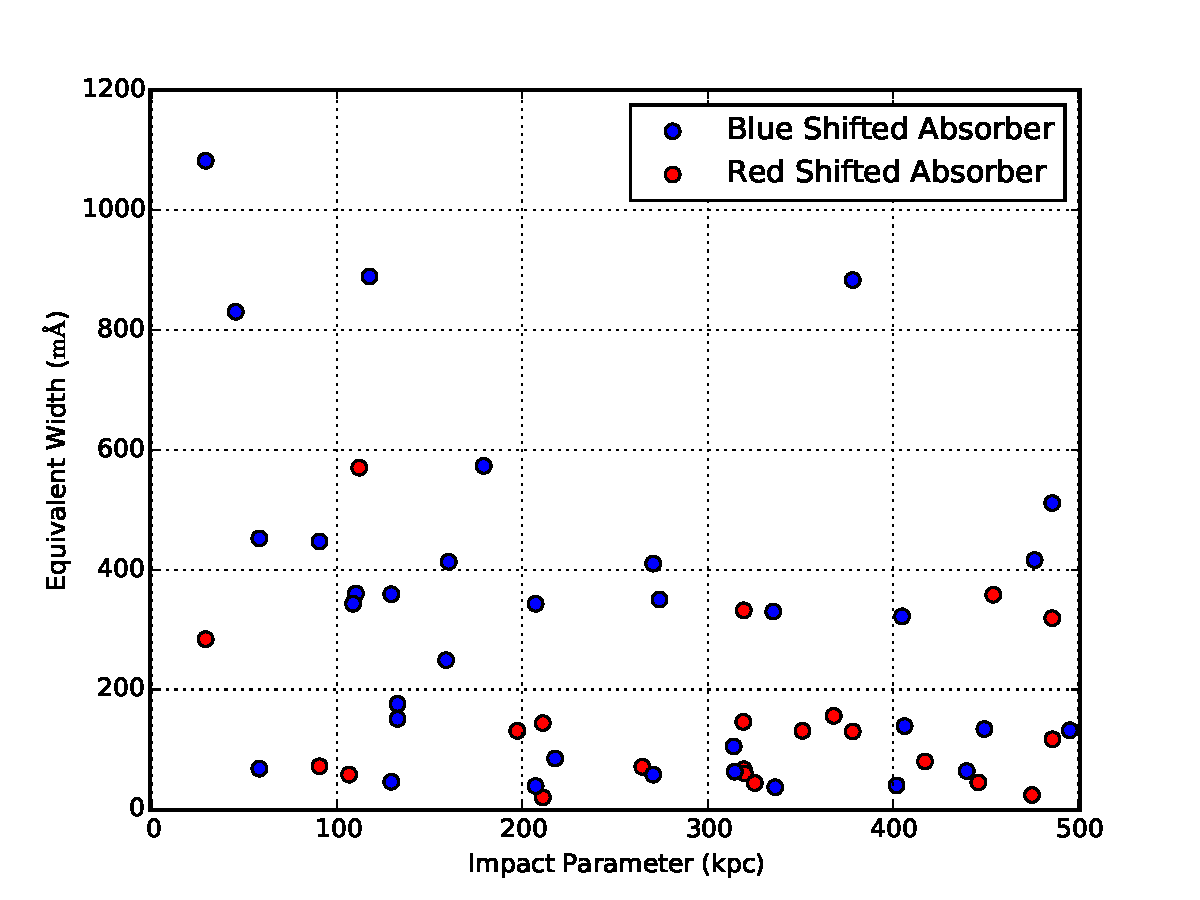
\includegraphics[width=0.52\textwidth]{W(impact)_dif.pdf}
%        \caption{\small{Equivalent width ($W$) of each absorber as a function of $\rho$ (kpc), the physical impact parameter between the galaxy and the sightline toward the absorption feature. Only a slight anti-correlation can be seen.}}
%        \label{ew_vs_impact}
%\end{minipage}\hfill
%\begin{minipage}[b]{.49\textwidth}
%        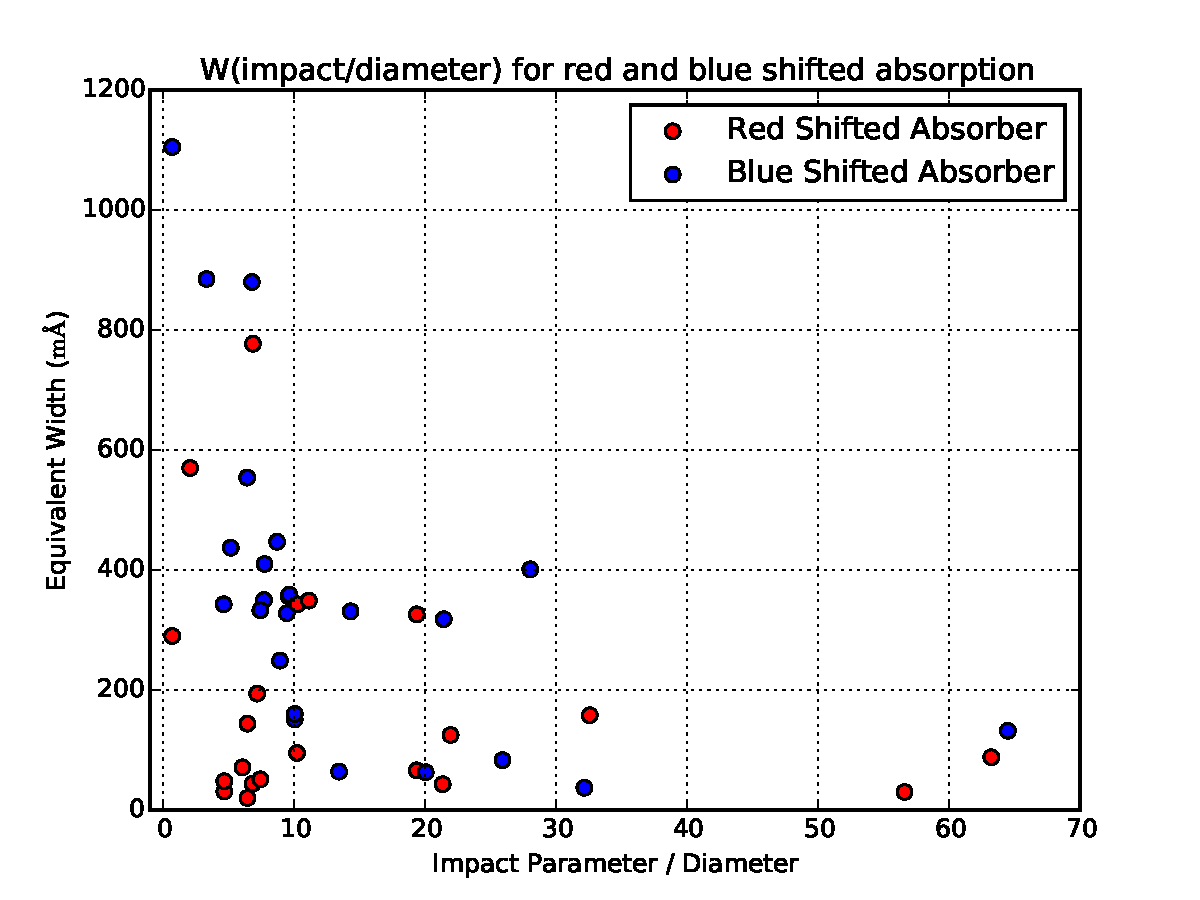
\includegraphics[width=0.52\textwidth]{W(impact_diam)_dif.pdf}
%        \caption{\small{Equivalent width ($W$) of each absorber as a function of $\rho$/D, the ratio of the physical impact parameter and the galaxy diameter. A strong anti-correlation is evident.}}
%%        \vspace{-5pt}
%        \label{ew_vs_impact-d}
%\end{minipage}
%\end{figure*}


%\begin{figure}[h!]
%        \centering
%        \vspace{-10pt}
%        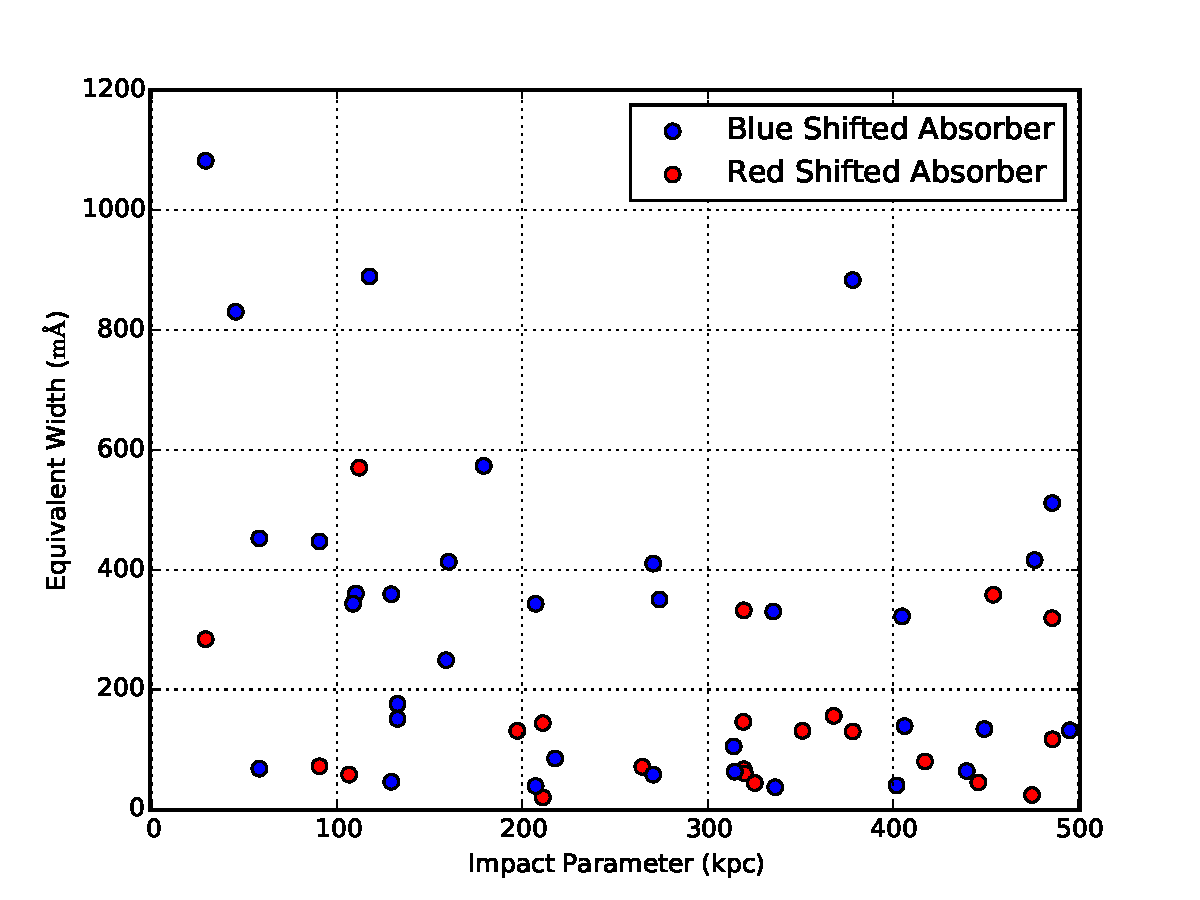
\includegraphics[width=0.52\textwidth]{W(impact)_dif.pdf}
%        \caption{\small{Equivalent width ($W$) of each absorber as a function of $\rho$ (kpc), the physical impact parameter between the galaxy and the sightline toward the absorption feature. Only a slight anti-correlation can be seen.}}
%%        \vspace{-5pt}
%        \label{ew_vs_impact}
%\end{figure} 
%
%\begin{figure}[h!]
%        \centering
%        \vspace{-10pt}
%        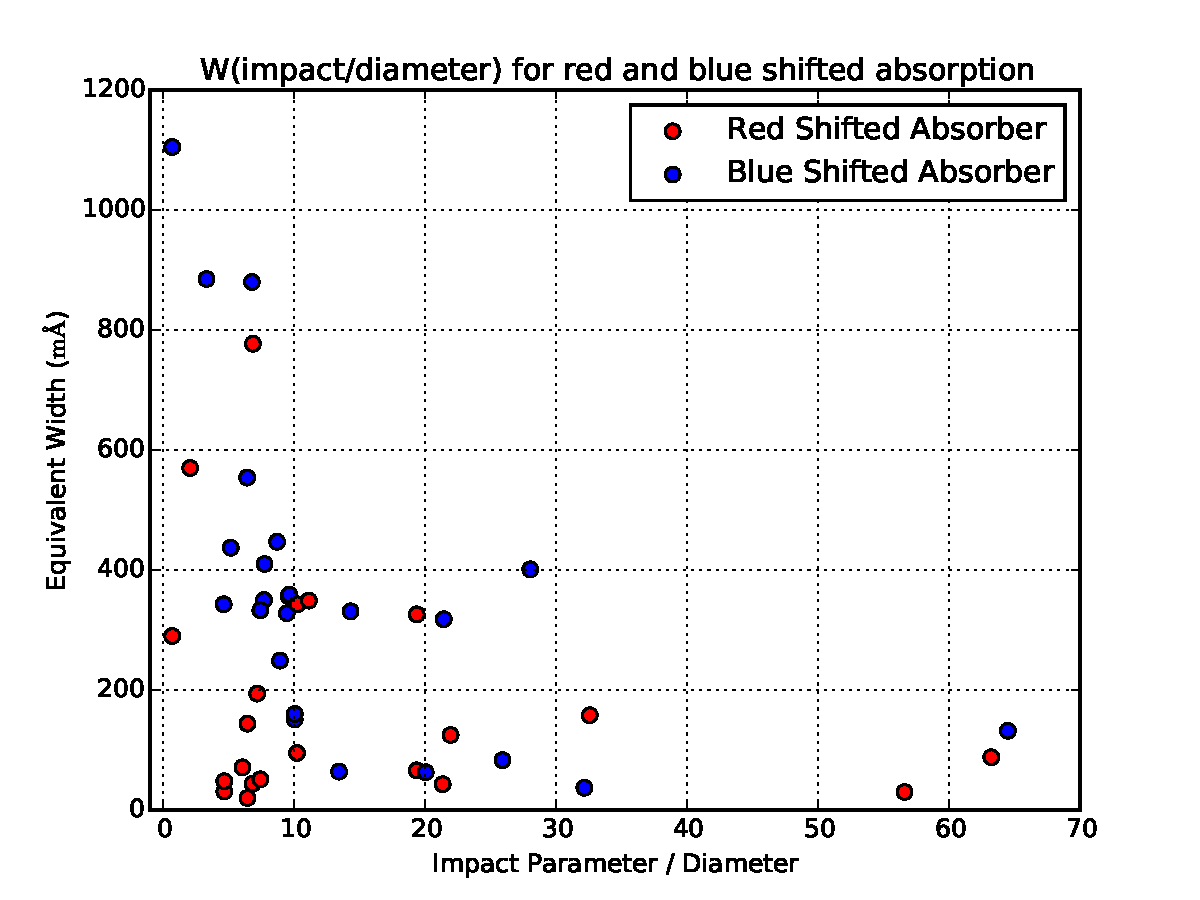
\includegraphics[width=0.52\textwidth]{W(impact_diam)_dif.pdf}
%        \caption{\small{Equivalent width ($W$) of each absorber as a function of $\rho$/D, the ratio of the physical impact parameter and the galaxy diameter. A strong anti-correlation is evident.}}
%%        \vspace{-5pt}
%        \label{ew_vs_impact-d}
%\end{figure} 


\begin{figure}[h!]
        \centering
        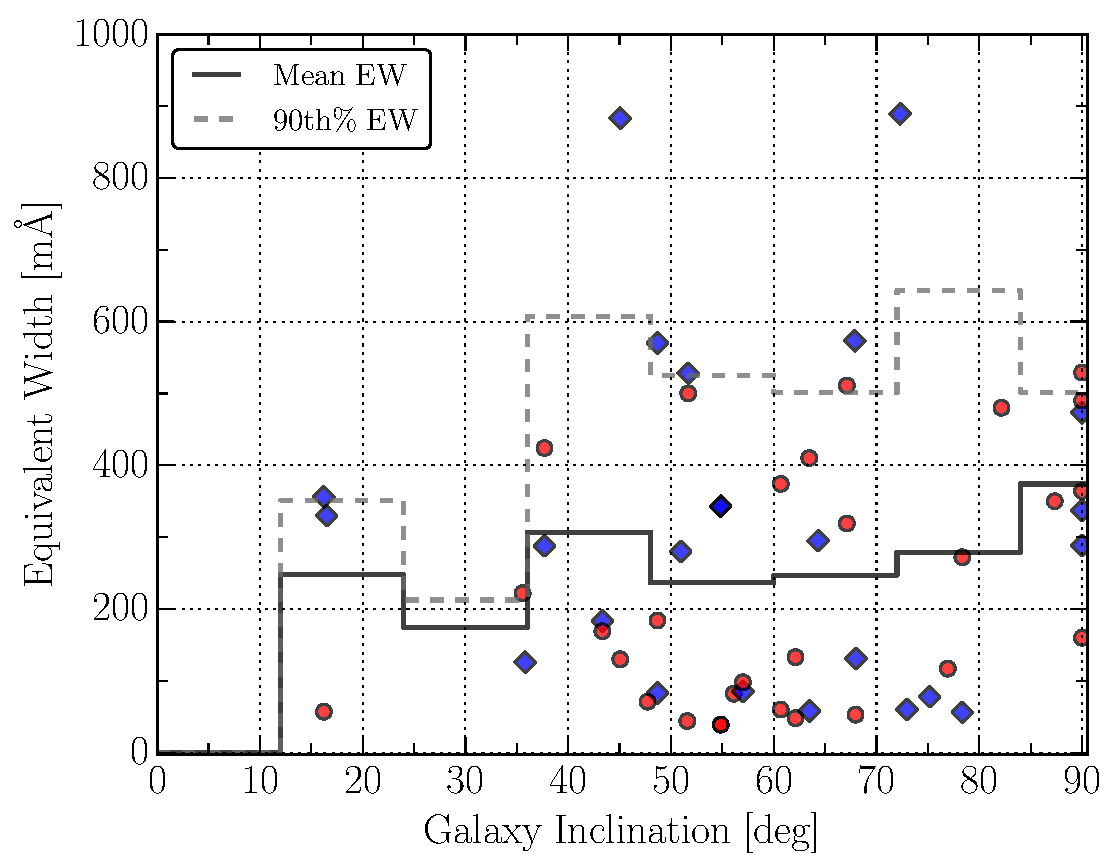
\includegraphics[width=0.48\textwidth]{W(fancy_inc)_mean_90_hist.pdf}
        \caption{\small{Equivalent width of each absorber as a function of the inclination angle of the associated galaxy. The dashed black line shows the mean $EW$ of all absorbers in bins of $15^{\circ}$.}}
        \label{ew_vs_inclination}
        \vspace{2pt}
\end{figure}

\begin{figure}[h!]
        \centering
        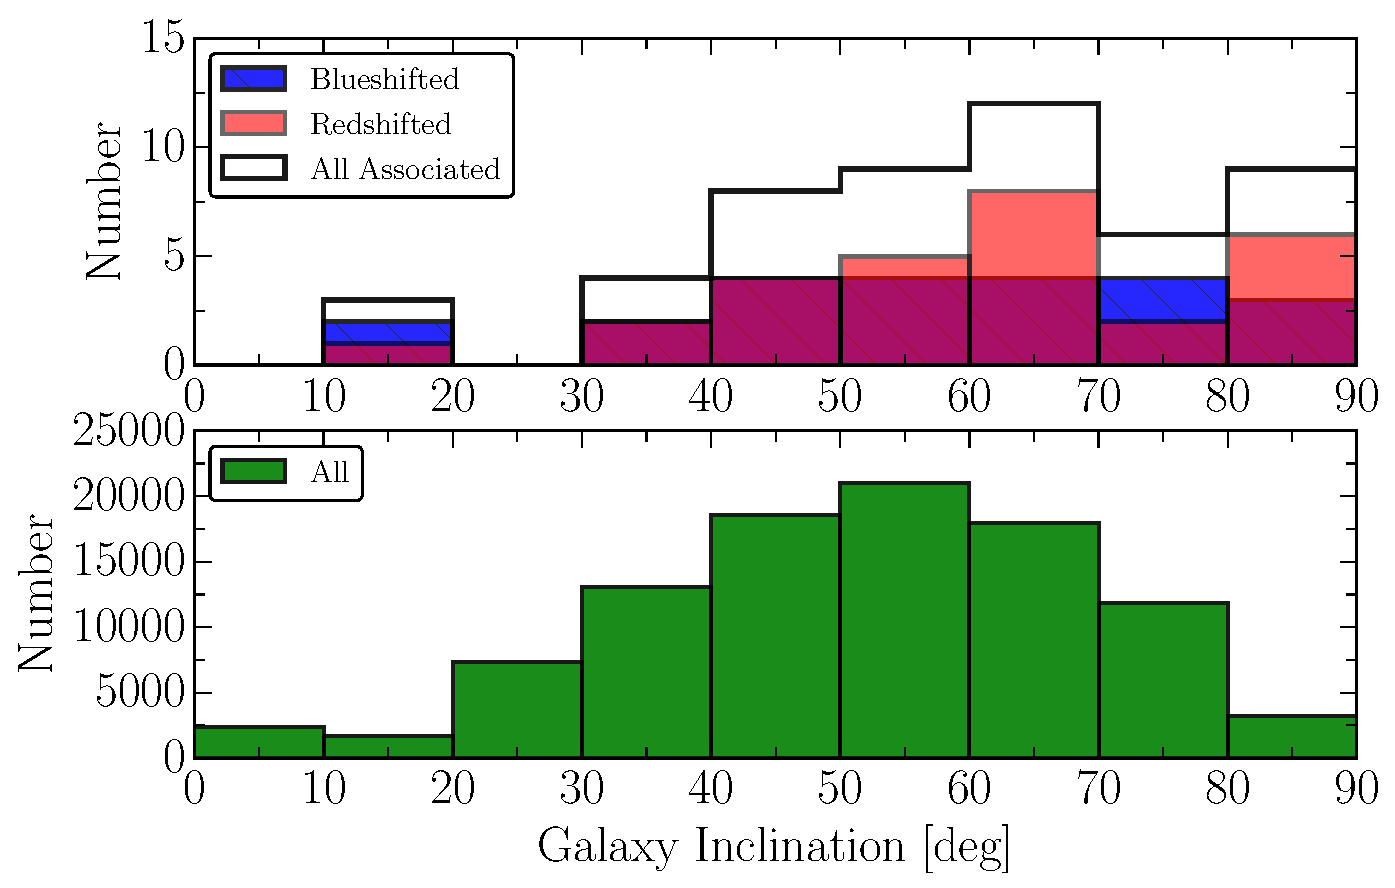
\includegraphics[width=0.48\textwidth]{hist(fancy_inclination)_red_blue_full_all.pdf}
        \caption{\small{\textbf{Top: }Distribution of inclinations for all associated galaxies, split into red and blue shifted sets. \textbf{Bottom:} Distribution of inclination of all galaxies in the $cz \leq 10,000$ km/s redshift range.}}
        \label{hist_inc}
        \vspace{2pt}
\end{figure}


\begin{figure}[ht!]
        \centering
        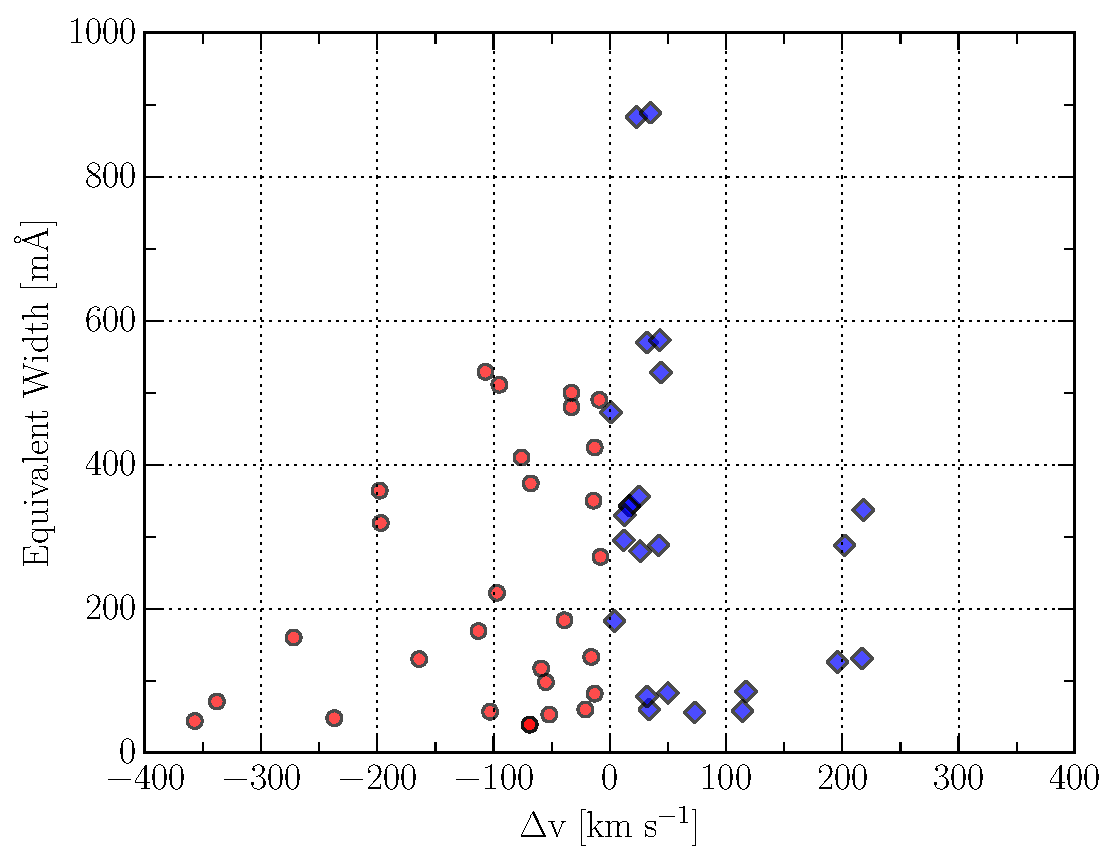
\includegraphics[width=0.48\textwidth]{W(vel_diff).pdf}
        \caption{\small{Equivalent width as a function of the velocity separation between the galaxy and absorption line.}}
        \label{W_veldif}
        \vspace{5pt}
\end{figure} 

\begin{figure}[ht!]
        \centering
        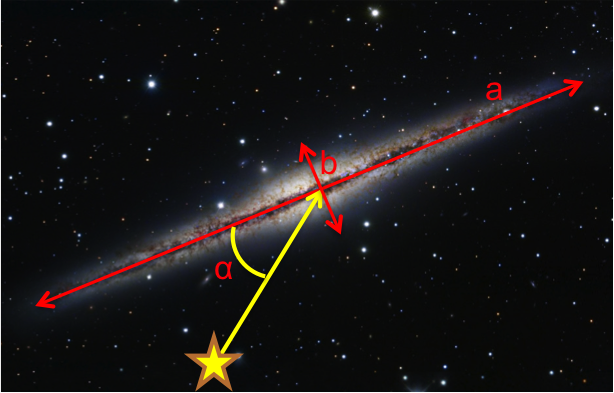
\includegraphics[width=0.48\textwidth]{azimuth_illustration2.png}
        \caption{\small{Azimuth is the angle, $\alpha$, between the major axis of the galaxy, $a$, and a vector extending from the AGN target to the galaxy center. Image of NGC891 credit: Composite Image Data - Subaru Telescope (NAOJ), Hubble Legacy Archive, Michael Joner, David Laney (West Mountain Observatory, BYU); Processing - Robert Gendler.}}
        \label{azimuth_illustration}
        \vspace{5pt}
\end{figure} 

\begin{figure}[ht!]
        \centering
        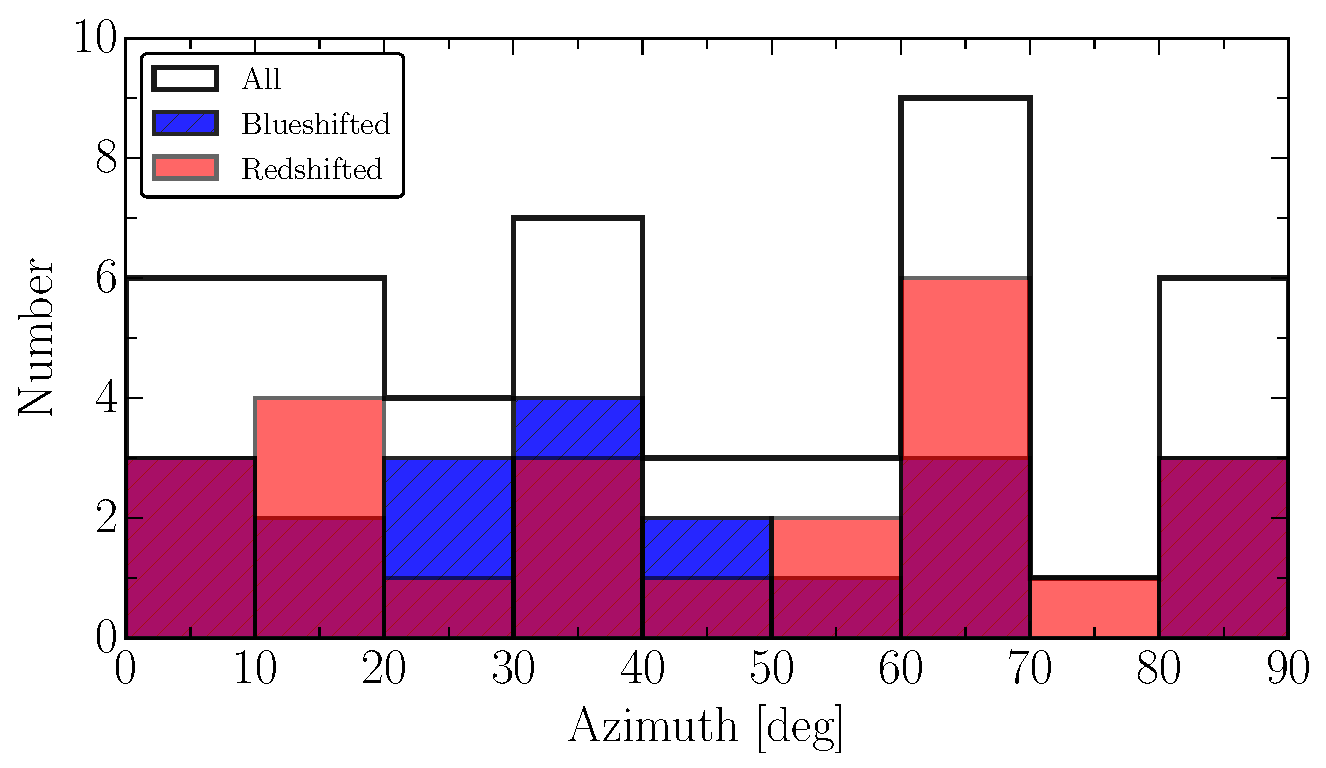
\includegraphics[width=0.48\textwidth]{hist(azimuth)_overlaid_all.pdf}
        \caption{\small{The distributions of azimuth angles for red and blue-shifted samples, with the combined sample plotted in black. $Azimuth = 0$ corresponds to along the projected major axis of the galaxy, and $azimuth = 90$ is along the minor axis.}}
        \label{azimuth_dist}
        \vspace{5pt}
\end{figure} 


\subsection{Inclination}
In this section we examine the inclinations of the associated galaxies compared to the distributions of absorbers. We correct for the finite thickness of galaxies, which causes $b/a$ to deviate from cos $i$ at high inclinations, by computing galaxy inclinations with the following formula from Heidmann et al. (1972a):

\begin{equation}
	\cos(i) = \sqrt{\frac{q^2 - q_0^2}{1 - q_0^2}},
	\label{incEq}
\end{equation}

\noindent where $q = b/a$, the ratio of the minor to major axis, and $q_0$ is the intrinsic axis ratio, set to $q_0 = 0.2$ for all galaxies (e.g., Jones, Davies, and Trewhella 1996). Only 5 of 

%Figure \ref{ew_vs_inclination} shows red and blueshifted absorbers' $EW$ plotted against the inclinations of their associated galaxies. We note that there is an apparent dichotomy between the distributions, where blue shifted absorbers appear around nearly all inclinations of galaxies, but redshifted absorbers appear preferentially near highly-inclined galaxies ($i \geq$ 50 deg). In addition, redshifted absorbers appear with lower $EW$ than those blueshifted across all inclinations. The mean $EW$ of all redshifted absorbers is $\overline{EW}$ = $237 \pm 16$  $\textrm{m\AA}$, compared to $\overline{EW}$ = $353 \pm 12$ $\textrm{m\AA}$ for blueshifted absorbers. To test if the distributions of red and blue-shifted absorbers are actually different we performed KS and AD statistical distribution tests, which both yielded p-values $=0.05$. While $p=0.05$ is often quoted as a threshold for significance, we believe a larger sample size is needed before we can claim the presence of a true, physical dichotomy.


Figure \ref{ew_vs_inclination} shows red and blueshifted absorbers' $EW$ plotted against the inclinations of their associated galaxies. We note that there is a clear excess of absorbers near galaxies of high inclination, with $75\%$ of redshifted and $65\%$ of blueshifted absorbers being associated with galaxies of $i \geq$ 50 deg. The solid-black and dashed-grey lines show mean and 90th percentile histograms, respectively, in bins of 12 deg. There does not appear to be much evolution of $EW$ across galaxy inclination, although a slight increase of mean $EW$ is possibly present towards higher inclinations. There are only 3 absorbers associated with a galaxy with $i<35$ 

In total $65\%$ of blueshifted and $75\%$ of redshifted absorbers are associated with high inclined galaxies ($i \geq$ 50 deg). Only $56\%$ of all galaxies in the survey volume are highly inclined, indicating a preference for detecting absorption around inclined galaxies. Figure \ref{hist_inc} shows the distribution of galaxy inclinations for both the red and blue-shifted associated galaxies and all galaxies within the survey volume. We tested the difference between the full distribution of inclination angles and the distribution for all (red + blue-shifted) associated galaxies using the Anderson-Darling (AD) and Kolmogorov-Smirnov (KS) statistical distribution tests, yielding p-values of $KS_{p} =0.0368$, and $AD_{p} = 0.00014$. Hence, there appears to be a significant bias towards detecting Ly$\alpha$ absorption around highly inclined galaxies. 

It is worth noting here that the observed distribution of galaxy inclinations is \emph{not} flat, as one might expect. Because our galaxy sample is essentially magnitude-limited, highly-inclined and optically thin galaxies can be detected out to larger distances and are thus over-represented in the sample (Jones, Davies and Trewhella 1996). It is possible that this effect is also responsible for the over-abundance of Ly$\alpha$ detections around highly inclined galaxies. If we assume a disky or oblate spheroid shape and some covering fraction for the CGM, the probability of encountering a cloud near an inclined galaxy would increase with the increased path-length through the halo. 


%It is important to note here that the majority of our sample of absorbers are measured far from galaxies (mean $\rho = 223$ kpc for blueshifted absorbers and $\rho = 290$ kpc for redshifted absorbers). Additionally, the differential velocity between galaxy and absorber ($\Delta v$) is on the order of the rotation velocity for spiral galaxies (average $\Delta v = 68$ km/s for blueshifted, $\Delta v = -102$ km/s for redshifted absorbers). Without further knowledge of the rotation velocity and orientation of each galaxy however, we can only speculate at the origins of the dichotomy between red and blue-shifted absorbers.

%In addition, redshifted absorbers appear with lower $EW$ than those blueshifted across all inclinations. The mean $EW$ of all redshifted absorbers is $\overline{EW}$ = $237 \pm 16$  $\textrm{m\AA}$, compared to $\overline{EW}$ = $353 \pm 12$ $\textrm{m\AA}$ for blueshifted absorbers. However, the results of KS and AD test do not assign a high significance to this result. 


\subsection{Velocity Difference \rm($\Delta v$\rm)}
%Additionally, we find evidence for an anti-correlation between absorber $EW$ and the velocity difference between the galaxy and the associated absorption, $\Delta v$. The mean and maximal $EW$ of absorption increases with decreasing $\Delta v$ (see Figure \ref{W_veldif}). In total, 25/41 ($61\%$) of absorbers are found within $\pm100$ km/s, and the highest $EW$ absorbers are found within $\pm50$ km/s  of their associated galaxy velocities.

We find evidence for an anti-correlation between absorber $EW$ and the velocity difference between the galaxy and the associated absorption, $\Delta v$. The mean and maximal $EW$ of absorption increases with decreasing $\Delta v$ (see Figure \ref{W_veldif}). In total, 35/51 ($69\%$) of absorbers are found within $\pm100$ km/s. This $\pm100$ km/s threshold also applies to absorber $EW$, with only 1 absorber of $EW \geq 400$ found with $\Delta v > 100$ km/s. Blueshifted absorbers are on average closer to their associated galaxy, with $\overline{\Delta v}_{blue} = 68$, compared to $\overline{\Delta v}_{red}=-102$ for the redshifted sample, and correspondingly have higher average equivalent width, $\overline{EW}_{blue}=317\pm18$ compared to $\overline{EW}_{red}=329\pm12$.

Additionally, of the 51 associated absorbers, 31 are matched with the same galaxy as another absorber (for a total of 15 unique galaxies in this subset). All but one of these cases involve two absorbers in the same sightline yet separated in velocity around a galaxy. 25/31 of these are oriented such that the higher $EW$ absorber has the smaller $\Delta v$, and the 6 others are close in either velocity or $EW$. The one galaxy with 3 associated absorbers, NGC1097, shows this trend across two sightlines as well, with absorbers at $\Delta v = 32$ km/s and $EW = 570$ $\rm m\AA$ towards 2dFGRS\_S393Z082, and $\Delta v = -39$ km/s and $EW = 184$ $\rm m\AA$ and $\Delta v = 50$ km/s and $EW = 83$ $\rm m\AA$ towards HE0241-3043.



\subsection{Azimuth}
In this section we examine properties of absorbers as a function of their azimuthal angle with respect to their associated galaxy. Azimuth is defined as the angle between the major axis of a galaxy and the vector connecting the absorption feature and the midpoint of the galaxy plane. Figure \ref{azimuth_illustration} illustrates this. 

The mean azimuth angle for blueshifted absorbers is $41^{\circ}$, and $45^{\circ}$ for redshifted absorbers. Figure \ref{azimuth_dist} shows the distribution of azimuth angles for both red and blue-shifted absorbers. Unlike the findings of Kacprzak et al. (2011, 2012), who find a bimodal distribution of Mg\,{\sc ii} absorbers around galaxies, our distributions of Ly$\alpha$ absorbers are generally consistent with a flat, or random distribution. There is a slight overabundance of absorbers around $0^{\circ}$ azimuth in both red and blue-shifted samples, but we cannot assign this observation much significance yet given the small sample size. We additionally find no significant correlation between azimuth angle and $EW$ or $\Delta v$. 

%Why would there be a preference for gas located blue-ward of galaxies, or equivalently, gas moving toward a galaxy from behind? If the gas is co-rotating, then this would mean that absorbers on the side of the galaxy moving toward us tend to be higher equivalent width clouds. What about infall vs outflows? Would infalling gas be higher equivalent width?


%\begin{table*}[ht]\footnotesize
%\begin{center}
%\begin{tabular}{l c c c c c c c c}
% \hline \hline
% $\Delta v$       &  \# of systems  &      Mean EW        &    Median EW      & Mean $\rm R_{vir}$ &   Mean $\rho$   &         Mean $\Delta v$            &    Mean Inc.        &  Mean Az.      \\ 
%  	                &                         & $\rm [m\AA]$        &   $\rm [m\AA]$    & \scriptsize [kpc]        & \scriptsize [kpc] & \scriptsize $\rm [km s^{-1}]$  & \scriptsize [deg] & \scriptsize [deg] \\
% \scriptsize (1)  & \scriptsize (2)  & \scriptsize (3)        &   \scriptsize (4)    & \scriptsize (5)           & \scriptsize (6)    & \scriptsize  (7)                        & \scriptsize (8)     & \scriptsize (9)      \\ \hline \hline
%
% Blueshifted     & 23                   & $317 \pm 18$        & $288 \pm 15$      &    210.7                    &   222.8               &        68                                   &    56                   &  41         \\
% \hline
% Redshifted      & 28                   & $239 \pm 12$        & $177 \pm 10$      &    221.3                    &  290.0               &       -102                                 &    59                   &  45    	\\
% 
%\hline
%\end{tabular}
%\end{center}
%  \caption{\small{Average properties of the associated galaxy sample split into red and blue-shifted bins based on $\Delta v$.}}
%  \label{resultsTable}
%\end{table*}



\section{Summary}


We have measured 51 $\rm Ly\alpha$ absorption lines in the spectra of 35 COS targets and matched each to a single, large ($D\geq 25$ kpc) galaxy. Table \ref{resultsTable} presents a breakdown of our results when separating absorber-galaxy pairs into red and blue-shifted samples. The following summarizes our findings:

\indent \textbullet \indent We introduce a likelihood parameter based on Gaussian profiles centered around $\rho / R_{vir}$ and $\Delta v$ to automate the matching of absorbers with associated galaxies. 

%\indent \textbullet \indent  Of our sample of 175 Ly$\alpha$ absorbers, only 41 can be unambiguously paired with a single nearby galaxy using our likelihood method. 46 absorbers are located near multiple galaxies and no definitive association can be made. The remainder, over half of the total sample, are located farther than 500 kpc and 400 km/s from a galaxy.

\indent \textbullet \indent $EW$ anti-correlates most strongly with $\rho$ when normalized by $R_{vir}$. It follows that $EW$ weakly correlates and anti-correlates with $R_{vir}$ and $\rho$, respectively.

\indent \textbullet \indent The mean and maximal $EW$ of absorbers increases with decreasing $\Delta v$. The strongest absorbers are nearly all found within $\Delta v = \pm 100$ km/s of their associated galaxies.

\indent \textbullet \indent We find a slight dichotomy in the $EW$ of absorption blue-ward vs red-ward of associated galaxies. Redshifted absorbers are weaker, with $\overline{EW}$ = $239 \pm 12$ $\textrm{m\AA}$ compared to $EW$ = $317 \pm 18$ $\textrm{m\AA}$ for blueshifted absorbers.

%\indent \textbullet \indent We find a positive correlation between the impact parameter ($\rho$) to the associated galaxy and $R_{vir}$ of said galaxy.

\textbullet \indent $\rm Ly\alpha$ absorbers are most associated with inclined galaxies. $65\%$ of blueshifted and $75\%$ of redshifted absorbers are associated with galaxies with $i \geq 50$ deg, whereas $56\%$ of all galaxies in the survey volume have similarly high inclinations. The distributions of associated vs all galaxy inclinations differ at a greater than $99\%$ significance level according to the Anderson-Darling distribution test.

\indent \textbullet \indent We find no strong azimuth preference for absorption - Ly$\alpha$ absorbers appear to be distributed uniformly around galaxies.


\begin{table}[ht]\footnotesize
\begin{center}
\begin{tabular}{l c c}
 \hline \hline
 Parameter                				&  Blueshifted   &     Redshifted        \\ 
  \hline \hline \\
  
 \# of systems          			 		&     	23				&	28			\\
 Mean $EW$    \scriptsize $\rm [m\AA]$    &	$317 \pm 18$ 		&	$239 \pm 12$  	\\
 Median EW     \scriptsize $\rm [m\AA]$    & 	$288 \pm 15$		& 	$177 \pm 10$	\\
 Mean $\rm R_{vir}$   \scriptsize [kpc]	&   	210.7			& 	221.3   		\\
 Mean $\rho$   \scriptsize [kpc]          		&   	222.8			& 	221.3		\\
 Mean $\Delta v$  \scriptsize $\rm [km s^{-1}]$     &	68				&	-102 			\\
 Mean Inc.  \scriptsize [deg]  			&  	56				&	59			\\
 Mean Az.  \scriptsize [deg]    			&	41				&	45			\\
   
\hline
\end{tabular}
\end{center}
  \caption{\small{Average properties of the associated galaxy sample split into red and blue-shifted bins based on $\Delta v$.}}
  \label{resultsTable}
\end{table}


\nocite{*}
\bibliography{paper_bib}
\bibliographystyle{apj}

\end{document}
